\documentclass[conference]{IEEEtran}
\IEEEoverridecommandlockouts
% The preceding line is only needed to identify funding in the first footnote. If that is unneeded, please comment it out.
\usepackage{cite}
% \usepackage{makecell}
\usepackage{hhline}
\usepackage{fancyhdr}
\usepackage[utf8]{inputenc}
\usepackage{amsmath,amssymb,amsfonts}
\usepackage{algorithmic}
\usepackage{graphicx}
\usepackage{textcomp}
\usepackage{blindtext}
\usepackage{pdfpages}
\usepackage{xcolor}
\usepackage{soul}
\usepackage{multirow}
\usepackage{booktabs}
\usepackage{array}
\usepackage{colortbl}
\usepackage{caption}
\usepackage{adjustbox}
\sethlcolor{yellow}

\def\BibTeX{{\rm B\kern-.05em{\sc i\kern-.025em b}\kern-.08em
    T\kern-.1667em\lower.7ex\hbox{E}\kern-.125emX}}
\fancyhf{}
\pagenumbering{arabic}
\cfoot{"pagenumber"}
% set table of contents depth to include sections and subsections
\setcounter{tocdepth}{2}

\begin{document}
\begin{titlepage}
    \begin{center}
        \vspace*{7cm}
        {\fontsize{16}{20}\selectfont Final Report} \\ 
        \vspace{.3cm}
        {\fontsize{16}{20}\selectfont Design 1} \\
        \vspace{.3cm}
        {\fontsize{16}{20}\selectfont Team 2}\\
        \vspace{.3cm}
        {\fontsize{16}{20}\selectfont Team 2: The Brain-Controlled Wheelchair} \\
        \vspace{.6cm}
        \textit{\fontsize{16}{20}\selectfont Gerhort Alford (C00058921)} \\
        \vspace{.3cm}
        \textit{\fontsize{16}{20}\selectfont Kaleb Guillot (C00405906)} \\
        \vspace{.3cm}
        \textit{\fontsize{16}{20}\selectfont April 3, 2023\\}
        \vfill
    \end{center}
\end{titlepage}
\thispagestyle{empty}
\pagestyle{empty}
\onecolumn
\tableofcontents
\twocolumn

\onecolumn
\clearpage
\thispagestyle{plain}
\pagestyle{plain}
\section*{\textbf{ABET Questions}}
\addcontentsline{toc}{section}{ABET Questions}
\begin{enumerate}
    \vspace{.6cm}
    
    \item \textit{How did this course provide you with an ability to identify, formulate, and solve complex engineering problems by applying principles of engineering, science, and mathematics?}
    \begin{itemize}
        \vspace{.3cm}
        \item Answer: This course gave us the ability to perform the scientific method for a problem that we have great interest in. We identified the problem, proposed a solution, performed research on related work, and are working to implement and experiment with the proposed solution. 
        \item Rank: 5
        \vspace{.3cm}
    \end{itemize}
    \item \textit{How did this course provide you with an ability to apply engineering design to produce solutions that meet specified needs with consideration of public health, safety, and welfare, as well as global, cultural, social, environmental, and economic factors?}
    \vspace{.3cm}
    \begin{itemize}
        \item Answer: With our design, there are many concerns to be addressed. These concerns not only include those addressed in the feasibility analysis, but also those which include safety of the user and a reliable and robust system. These problems have been weighed by the team, and solutions have been proposed through both software and hardware implementation. 
        \item Rank: 5
        \vspace{.3cm}
    \end{itemize}
    \item \textit{How did this course provide you with an ability to communicate effectively with a range of audiences?}
    \begin{itemize}
        \vspace{.3cm}
        \item Answer: This course provided the team with opportunities to present and communicate our ideas on a weekly basis to the class as well as to a wide range of audiences for E\&T Week.
        \item Rank: 5
        \vspace{.3cm}
    \end{itemize}
    \item \textit{How did this course provide you with an ability to recognize ethical and professional responsibilities in engineering situations and make informed judgments, which must consider the impact of engineering solutions in global, economic, environmental and societal contexts?}
    \begin{itemize}
        \vspace{.3cm}
        \item Answer: For a project aimed at assisting those less physically able, safety was the top priority. While this project aims at building a proof-of-concept, a product of similar nature must be reliable in all weather conditions and have protection from any malfunction or misuse.
        \item Rank: 4
        \vspace{.3cm}
    \end{itemize}
    \item \textit{ How did this course provide you with an ability to function effectively on a team whose members together provide leadership, create a collaborative and inclusive environment, establish goals, plan tasks, and meet objectives?}
    \begin{itemize}
        \vspace{.3cm}
        \item Answer: Through working on a team in which each member brought their own set of strengths and weaknesses, the work was able to be effectively delegated between them and the goals were able to be achieved.
        \item Rank: 4
        \vspace{.3cm}
    \end{itemize}
    \item \textit{How did this course provide you with an ability to acquire and apply new knowledge as needed, using appropriate learning strategies?}
    \begin{itemize}
        \vspace{.3cm}
        \item Answer: The project was an entirely new forte for the team. It requires both members to reach out to peers and experts for advice as well as intensely research related subjects.
        \item Rank: 5
        \vspace{.3cm}
    \end{itemize}
\end{enumerate}
\twocolumn


\title{The Brain-Controlled Wheelchair{\footnotesize \textsuperscript{*}}
\thanks{This project was submitted for review on February 13, 2023. The project mentor and sponsor is Dr. Magdy Bayoumi. G.M. Alford is with the Electrical and Computer Engineering Department, University of Louisiana at Lafayette, LA 70504 USA (email: c00058921@louisiana.edu).\\K. J. Guillot is with the Electrical and Computer Engineering Department, University of Louisiana at Lafayette, LA 70504 USA (email: C00405906@louisiana.edu)}
}
\author{

\IEEEauthorblockN{Gerhort M. Alford, \textit{Student Member, IEEE} and Kaleb J. Guillot, \textit{Student Member, IEEE}}
% \IEEEauthorblockA{\textit{Member, IEEE} 
% \textit{}
% City, Country \\
% email address or ORCID
}

\maketitle
\thispagestyle{plain}
\pagestyle{plain}
\vspace{-7mm}

\begin{abstract}
Developed by Gerhort M. Alford and Kaleb Guillot with All Rights Reserved. This paper presents the development of a proposal for an additional layer of control for a motorized wheelchair. This layer involves a BCI* in which the user will steer the wheelchair through focused thought. The interface will utilize an EEG* cap equipped with electrodes touching the user's scalp to gather signals emanating from the brain. Noise filtration will be performed by the cap's onboard processor. The filtered signal will then be sent to a minicomputer equipped on the wheelchair. The minicomputer is responsible for orchestrating operations, taking inputs and transmitting outputs to direct wheelchair movement. To distinguish signals from the EEG cap, a machine learning model will be employed. During testing, this model will temporarily be offloaded to a server, transmitting the signals via WiFi. Once the effectiveness of the model is verified, work will be done to implement the algorithm on an FPGA*, allowing the signal to be decoded locally. The brain commands to steer the wheelchair will involve MI*, where the user will imagine moving different parts of their body to correspond to wheelchair movement. The paper provides a comprehensive overview of the proposed design, including a timeline, potential safety concerns, and a cost analysis. The paper will explore alternatives to the design, including types of EEG headsets, signal processing hardware, and external sensors. The trade-offs associated with each alternative will be carefully considered and evaluated to determine the most viable option. This project will demonstrate the potential to improve mobility for those with physical limitations through use of non-invasive BCI.
\end{abstract}

\begin{IEEEkeywords}
motor-imagery (MI), brain-computer interface (BCI), brain-machine interface (BMI), electroencephalogram (EEG), field programmable gate array (FPGA)
\end{IEEEkeywords}
\renewcommand{\thesubsection}{\Roman{section}.\Alph{subsection}}
\section{Introduction}
    The ability to move and live independently is a privilege that many take for granted. For millions of people around the world, physical limitations have made it challenging to operate a motorized wheelchair on their own. This leaves a significant number of people in need of further assistance from caregivers, decreasing feelings of independence and overall quality of life. Estimates indicate that between 1.4 and 2.1 million wheelchair users might benefit from a smart-powered wheelchair if it were able to provide a degree of additional assistance to the driver \cite{smart_wheelchairs}.  
    
    Impaired mobility has numerous downfalls. Psychologically, a decrease in independent mobility is associated to feelings of emotional loss, reduced self-esteem, isolation, stress, and fear of abandonment. In one's life, impaired mobility often decreases opportunities to socialize, resulting in social isolation, anxiety, and depression \cite{how_many_people}.
    
    Brain-Computer Interfaces (BCIs) are systems that allow the translation of real-time activity of the brain into commands that control devices. They rely solely on brain waves and can therefore provide a level of control for a device to a user suffering from a devastating neurodegenerative disorder \cite{noninvasive_brain}.

    In the last few years, BCI neurobiotic prototypes have flourished. Both invasive (implanted) and non-invasive (headset) approaches have produced devices such as robotic arms, exoskeletons, wheelchairs and telepresence robots \cite{learning_to_control}. In these devices, invasive BCI Systems much better signal to noise ratios due to the devices being implanted as close to the sources of the signals as possible. However, due to the portability, time constraints, and budget, electroencephalography (EEG) is a viable non-invasive option for this team's use. EEG uses electrodes placed at the scalp to retrieve brain signals, offering a view of multiple brain regions as well as high temporal resolution \cite{toward_brain_computer}.
    
    This paper proposes a solution for those unable to independently operate a motorized wheelchair - a brain-controlled wheelchair. This design utilizes a BCI system to translate real-time brain activity into commands that control the movement of a motorized wheelchair. This proposed model will work by using an EEG headset interfaced with a processing unit that will determine if the incoming signals dictate the movement of the wheelchair in a particular direction. To move, the processor will send signals to a motor controller that drives the movement of the electric motors. 
    
    To process the signals collected from the EEG cap, machine learning will be used to classify these signals into specific commands. There are six proposed categories of classification: forward, backward, left, right, stop, and none. The goal of the project is to process the signals locally, offloading the repetitive machine learning calculations to an onboard FPGA. However, for testing and verifying the model's effectiveness, the calculations will be offloaded to a remote server communicating with the onboard minicomputer via WiFi. 

    EEG signals themselves are not able to encapsulate the subtle movements that a wheelchair needs to accomplish. They can be decoded into commands like "forward," "backward," "left," and "right," but then the system is left to decide to what intensity to execute these commands. Does the user want to completely turn around or simply turn a few degrees? As the authors in \cite{learning_to_control} describe, the machine receiving the signals is akin to a passenger in a car giving a driver directions to a destination. The passenger does not need to tell the driver exactly how much force to apply to the accelerator and the brake; the driver is intelligent enough to make minute decisions. In the application of this project, the system requires a substantial amount of artificial intelligence to make context-based decisions. This will also help make the system safer to the user. Any error made while controlling the wheelchair, whether an accident from the user or a malfunction from the machine, may endanger the user. For these reasons, the system will be equipped with shared-control strategies. These are preventative measures instilled, such as sensors, lasers, or cameras, that will prevent collisions and regulate speed when approaching an object \cite{toward_brain_computer}. 
    
    Independent mobility increases opportunities in one's life, including educational and vocational \cite{how_many_people}. With the completion of this project, a step will be made in the direction of a more inclusive and well-rounded society.

\section{Related Work}
Brain-Controlled wheelchairs have been prevalent in research since the late 2000s. BCI wheelchairs fall into the larger category of smart wheelchairs (SWs), which are power wheelchairs (PWs) equipped with sensors, computers, and other assistive technologies \cite{a_comprehensive_review}. SWs have been under research since the middle of the 20th century, however, in recent years, the need for a device that accommodates a wider audience has remained while the research has unfortunately lost prevalence.  

    \subsection{Early Work}
    The development of PWs for individuals suffering from quadriplegia can be traced back to George Klein, who began his research following World War II. Prior to this time, individuals with quadriplegia were confined to their beds due to the limited technology available and were unable to lead fulfilling lives. In response to Klein's research, the American Wheelchair Company and Everest \& Jennings began producing PWs for mass distribution in 1956 \cite{a_comprehensive_review}. While these wheelchairs provided a degree of independence and improved the quality of life for many individuals with quadriplegia, they were not ideal for all patients and often required extensive safety modifications and improvements to increase comfort.

    Recognizing this issue, Dr. J. Leaman sought to create a more inclusive design for PWs in the late 1990s \cite{a_comprehensive_review}. At this time, many SWs were essentially mobile robots with attached seating, resulting in large form factors that made them impractical for everyday use. There were numerous types of input methods for these wheelchairs, including voice recognition, sight path detection, and computer vision \cite{smart_wheelchairs}. However, the primary drawback of these designs was the requirement for user supervision, as they did not accommodate individuals who were physically unable to control the chair through other means. For example, early SWs were only semi-autonomous, relying on user inputs such as a final destination or collision avoidance and leaving the navigation duties entirely up to manual input \cite{smart_wheelchairs}. 
    
    \subsection{Beginning of the Brain controlled wheelchair}
    Dr. Leaman finalized his invention in 2007, dubbed the iChair. This chair's movement was accomplished through a combination of a head tracking mouse and a Mount-n-Mover \cite{a_comprehensive_review}. In 2009, the authors of \cite{noninvasive_brain} took this a step further, using P300 neurophysiological protocol where the user would steer the wheelchair by concentrating on a certain section of the user interface. The advancement of this project was the use of computer vision. When the route for the wheelchair was selected by the user, the wheelchair would automatically drive to the destination. This took much of the mental strain involved out of the equation. Though, this system was not perfect; it suffered from the flaw of low information transfer rates, making instantaneous feedback impossible.  
    
    \subsection{Recent Years}
    In the past decade, there has been more attention towards developing reliable, noninvasive brain-controlled wheelchairs \cite{learning_to_control, self_paced, robotic_architecture, toward_brain_computer, biomedical-signal}. In 2012, the authors of \cite{self_paced} developed a system with a similar goal to this project, and with similar hardware. They employed the EMOTIV EPOC to gather brain signals and tasked the subject with performing motor-imagery (MI) tasks in order to steer the wheelchair. However, the headset was far too sensitive to noise and produced far too many false positives. In the following year, the authors of \cite{robotic_architecture} used a shared control architecture utilizing robotic perception and computer vision-based obstacle detection for an asynchronous approach to the concept. More recent projects have followed along with a shared control architecture, with the authors of \cite{learning_to_control} using integrated sensors to allow for external, computer based control to gather information about the surrounding environment to ensure user safety. This paper used a 32 channel ANT Neuro to compute a user's intent using the short-time direct directed transfer function (SdDTF). Other implementations took slightly different routes while still using similar technology. The authors of \cite{toward_brain_computer} used a virtual environment to test their implementation which involved a user focusing on one of many particular sensors connected to various parts of the user's body to move the wheelchair in a specific direction. 

    \subsection{Shared-Control Strategies}
    The broader category of brain-machine interfaces (BMI) employ hardware components and software protocols that protect both the user and the system itself. The components included in shared-control strategies take responsibility and strain away from the user and allow the system to handle the minute details. In \cite{robo-teleop}, mobile robots were controlled via EEG signals and protected with shared intelligence systems. These systems included software policies for obstacle-avoidance, measuring distance, accounting for user input, changes of direction, and a fusion of all four. The hardware employed included a laser range finder for obstacle detection and a 3-D camera. As one can imagine, this stragegy is very computationally intense, as this project required an embedded PC and onboard laptop.  

    In \cite{learning_to_control}, a brain-controlled wheelchair is employed and tested on participants affected with severe tetrapalegia. The term "mutual learning" is adopted to describe the closed loop control that improves brain signal modulation through feedback and their BMI decoder model that infers the underlying mental task from incoming brain signals after data-driven parameter estimation. Mutual learning allows the decoder to gain accuracy over time in both understanding the user's given command as well as interpreting the intended intensity behind the command. For example, if the decoder interprets that the user has been giving the command to turn left for some time, and the wheelchair is in a hallway where the only options to move are forward and backwards, then the decoder may decide that the user wishes to turn around. The authors of this paper incrementally re-calibrated the encoder based on the performance of the BMI. 

    \subsection{Machine Learning Strategies}
    To correctly classify incoming EEG signals, it is imperative to adequately employ a well documented and researched model. This model has to work accurately and reliably while remaining computationally inexpensive so as to characterize signals in a time efficient manner.  

    In recent years, one of the most common deep learning models has been the use of Long Short-Term Memory (LSTM) blocks. These blocks are implemented on EEG-Based signals for MI classification in \cite{lstm_eeg}. The authors first decompose the incoming signals into their respective frequency bands: alpha, beta, theta, and delta. The LSTM blocks are used as multi-class classifiers and combined with softmax layers for motion intention classification. This methodology displayed high accuracy, but was computationally intense. 

    A more simplistic network suitable for this project is the Convolutional Neural Network (CNN). The authors of \cite{deep_learning_eeg} compared five different deep learning models or EEG classification, with four of the five being CNNs. The experimenters measured the accuracy, training time, and inference time of each model while also comparing the effectiveness of each model from subject to subject. They concluded that EEGNet was, on average, the best performing, sporting a high accuracy and low inference time. However, they remarked that the inter-connectivity of the deep learning model varied heavily from subject to subject, remarking that different connective structures performed better or worse on select subjects. 

    EEGNet is designed to be computationally efficient, having fewer parameters than other deep learning models. It uses depth-wise separable convolutions to reduce the number of parameters while maintaining a high accuracy \cite{eegnet}. This model is promising for use of this project, as the model has been implemented on portable hardware in \cite{eegnet_processor_design}. This would be beneficial for an eventual FPGA implementation. 

    For improved accuracy in EEG-based motor imagery classification, the authors of \cite{dmtl_bci} propose an end-to-end learning strategy. The authors propose a novel model, named DMTL-BCI, wherin features are learned from raw signals automatically and the feature extractor and classifier are optimized simultaneously. Their proposal consists of three modules: the representation module, the reconstruction module, and the classification module. These modules are interconnected and share intermediate features, enhancing the generalization ability of the model and improving the performance of the classification with limited data. This is relevant to applications of this project, as the dataset for a given individual will be limited, and high accuracy is crucial for overall performance of the system. 
    

\section{Project Analysis}
    \subsection{Feasibility Analysis}\label{}

    %%%%%%%%%%%%%%%%%%%%%%%%%%%%%%%%%%%%%%%%%%%%%%%%
    From the team's research, multiple other projects have been found that have constructed a brain-controlled wheelchair using an EEG cap and have then used methods of either digital signal processing \cite{noninvasive_brain} or a combination of signal processing and machine learning to interpret the signal \cite{a_comprehensive_review, learning_to_control, robotic_architecture, toward_brain_computer}. The technological feasibility of this project will be divided into the different components that will be used to build the brain-controlled wheelchair and software. To control the motorized wheelchair, the planned component is an EEG cap from OpenBCI, the Ultracortex Mark IV Headset. This headset is responsible for sending raw EEG signal data to a minicomputer on the motorized wheelchair. The computational requirements for the minicomputer {is presently not known as the team has not yet reached a conclusion on the chosen machine learning model. The team may also take the alternative route of offloading the processing to a server. In this case, the onboard minicomputer would serve to collect, transmit, receive, and then output data.} Multiple models will be constructed and consequently trained on online data sets containing similar data to that of what is collected from the Ultracortex. These models will range from simple classification to the more complex, such as an RNN with LSTM blocks capturing temporal locality. After sufficient training and testing, the model will be selected. {If the team chooses to not offload the machine learning computations, a compromise will need to be reached between model accuracy and hardware capability.} 
    
    While the software model is being developed and tested, the group will work on data acquisition with the Ultracortex. This will work through subjects using motor imagery (MI) thoughts, where a user wearing the cap will focus on objects in their view and then concentrate on a particular direction to move said objects. The onboard processor will take the input of the EEG signals, and output signals to motor drivers connected to the motors controlling the wheels of the wheelchair. If time permits the machine learning model will be implemented using an FPGA for faster and more efficient processing. Translating a machine learning model to run on an FPGA, while not simple, is fully possible, as shown in \cite{fpga_intel}. Motorized wheelchairs are easily accessible and commercially available. In this project, the team plans to design their own motorized wheelchair; beginning with a standard manual wheelchair and then attaching motors and other necessary components. This motorized wheelchair will only be for testing purposes and will not be a final product. The main goal of mentor and sponsor Dr. Magdy  Bayoumi is to have the working machine learning model and hardware implementation done. From a technological perspective, this project is feasible.  
    %%%%%%%%%%%%%%%%%%%%%%%%%%%%%%%%%%%%%%%%%%%%%%%%
    
    % \subsection{Time Feasibility}
    The section of this project that is expected to be the most time-consuming will be handling and preprocessing the data. This task is delegated evenly between the two group members: Kaleb Guillot will code various machine learning models in python and use open source datasets to train the models to test for effectiveness. Both group members will then select a single model that balances effectiveness with complexity. Kaleb Guillot will then code the selected model in C, and then use toolkits to translate the model onto an FPGA. During this Gerhort Alford will work with the Ultracortex to perform data acquisition. Gerhort Alford will record EEG signals while performing MI tasks and will then preprocess the signals. This step will include noise filtration and feature selection and is expected to be very time-consuming. When Kaleb Guillot finishes coding a machine learning model in C, he will then move to assist Gerhort Alford with preprocessing the EEG signals from Gerhort Alford. Once the software implementation has been completed, the next step will be interfacing with the hardware of the motors. This task will primarily be handled by Gerhort Alford, however, assistance will be provided by Kaleb Guillot when needed. The length of time given for this project has been deemed feasible as project mentor and sponsor Dr. Bayoumi's main goal for us is to implement an effective machine learning model that decodes EEG signals. A Gantt Chart will be used to make sure progress is kept on time.
    
    
    % \subsection{Financial Feasibility}
    After compiling a list of parts required and speaking with project mentor and sponsor Dr. Magdy Bayoumi, the team has deemed this project financially feasible. Most of the components required for this project have already been obtained and most of the software required for this project has no cost. The raspberry pi 4, motor controllers, electric motors, and chair component costs are well within Kaleb Guillot's originally proposed budget of up to \$7,550, which has been approved by Dr. Bayoumi.  
    
    % \subsection{Legal Feasibility}
    The final consideration for the feasibility of this project is legal feasibility. The team plans on using noninvasive techniques of reading a user's brain signals so this project does not involve any medical procedure to take place on the user. Though wheelchairs do fall under Food and Drug Administration FDA and possibly Americans with Disabilities ACT ADA, in terms of this project, the goal is to build an initial prototype that can then be modified later to meet the requirements of the FDA and ADA. Guaranteeing reliable output and the safety of all users will be the main consideration when designing the final implementation. This test wheelchair will only be for initial testing not the final product. Legally, this project has been deemed feasible as the team will not be dealing with the aspect of the project that would require legal attention as this will mainly be the initial groundwork to be expanded upon later. 

    \subsection{Alternatives and Trade-offs}
    This project has been broken down into three sections: obtaining EEG signals, processing the signals, and translating the results into movement. The main consideration is the processor that will process the signals from the EEG cap. After discussion with the team, the likely option will be a Raspberry Pi 4 8GB model with the TUL Pynq Z2 FPGA as a signal processor. However, this is subject to change, as a working machine learning model must be chosen before choosing an adequate processor. The Raspberry Pi will serve to easily interface with the motor drivers, manual controls, and user displays. The FPGA will take on the task of the processing the signals from the EEG cap as it should be much faster at this task. Both these items are already on hand, so testing with them can begin as soon as the machine learning model is trained and team member Gerhort Alford has done research with the TUL Pynq Z2 FPGA.

    Another proposed option was to use the Raspberry Pi 4 8GB model with a Tensor processing unit. The Raspberry Pi will work as in the previous option with the FPGA but the Tensor processing unit will take on the task of processing the brain signals quickly. This option will be favored if the FPGA implementation of the machine learning model proves to be unrealistic due to hardware resource limitation and budget.  

    To acquire the signals, multiple EEG caps from multiple different companies have been considered. These companies are EMOTIV, OpenBCI, and G.Tec. EMOTIV creates headsets that are very easy to use and have eye-catching features. EMOTIV headsets are suitable for beginners to the field who only want to monitor EEG signals, performing well in areas such as psychology. These headsets are not suitable for engineering applications. To simply view the raw EEG signals, a special, expensive, yearly license is required. The EMOTIV headsets also have electrodes that are fixed in place, not allowing the experimenter to choose electrode placement through testing. OpenBCI headsets are designed with the engineering perspective in mind. They have fully open-source software and their hardware is highly configurable. Headsets can be taken apart, electrodes can be moved around, and raw data can be manipulated. This company makes it possible for the buyer to design their own headsets to support OpenBCI's electrodes using 3-D printing. G.Tec headsets take configuration to the next level, however the majority of this configuration is handled through preference selection on their website and then implemented by the company itself, rather than fully handled by the buyers as in the case of OpenBCI. These headsets are suitable for serious research projects, with the price tag reflecting their quality. G.Tec produces the headsets of choice of the authors of \cite{learning_to_control}, the inspiration for this project. After consideration, the group elected to use an Open BCI headset, specifically the Ultracortex Mark IV. This headset has both a reasonable price and a good reputation in the research community \cite{openbci-research}.
    
    When translating a brain signal into movement, there are several intermediate steps between decoding the EEG command and moving the wheelchair. An analogy can be made to giving directions to the driver of a car. When telling the driver where to go, general directions will be given such as "turn at the next light" or "make a u-turn." The driver will handle the minute movements of the car, e.g, applying the brake, or making sure that is is safe to make the u-turn. This same concept applies to a brain-controlled wheelchair. The user acts as the passenger, giving the wheelchair general directions. The wheelchair needs to decide for itself when and how to make the precise movements to allow for a same and smooth ride. These movements, sometimes referred to as computer vision, are made through processing sensor information about the environment surrounding the wheelchair. The sensors will be mounted on each of the four sides, allowing the wheelchair to gather a more complete picture and make an informed decision. The group has considered several different types of sensors, including ultrasonic, infrared, laser light (LIDAR), and cameras. Each provides its own set of pros and cons, but the group has opted for a combination of ultrasonic and infrared sensors due to their low cost and required processing power.  
    
    More details of alternative and trade-off analysis can be found in Appendix C. 

    \subsection{Preliminary Design}
    This section outlines the necessary components and their roles in the project. The responsibilities of the hardware and software are analyzed from the perspective of the component's functionality as well as their contribution to the system as a whole. Diagrams, flowcharts, and Failure Modes and Effects Analysis (FMEA) were used to analyze the project. More details of the preliminary design can be found in Appendix D. This section aims to provide a comprehensive overview of the design process and the steps taken to ensure that the final product meets the project's objectives.
    
    The Brain-Controlled Wheelchair involves using powerful hardware, an open-source EEG cap, and robust software to accomplish the design goal. The hardware chosen for this task includes an Orange Pi 5 16 GB RAM model, TUL Pynq Z2 FPGA, OpenBCI Ultracortex Mark IV EEG cap, two stepper motors, a stepper motor controller, two rotary photo encoders, ADS1115 16-bit analog-to-digital converter (ADC), a joystick, and the necessary components to implement a shared-control between the user and the wheelchair. The hardware used to implement computer vision includes a combination of infrared and ultrasonic sensors mounted at specified points on the wheelchair. To develop this project, coding will be done in Python and C/C++, using libraries from OpenBCI and Google to process data. Other software used for modeling includes Vivado and Onshape. When the FPGA is implemented to handle the repetitive calculations of the machine learning model, the code for the hardware will be written in Verilog.

    The project will begin by using the EEG cap to acquire a signal. The team will collaborate to build a dataset, pre-process the signals, and construct the machine learning model. Once the effectiveness of the model is verified, the onboard minicomputer will offload the repetitive parallel calculations to an FPGA. The output from the model will be used to command the motor controller. The team plans to conduct multiple testing phases, including using LEDs to monitor output, interfacing the headset with a miniature remote-controlled (RC) car, and finally, testing the proof-of-concept wheelchair. The team recognizes that building a complete motorized wheelchair for public use is outside of their scope of work. As a result, some common safety and quality of life features of normal motorized wheelchairs will be omitted. The team will still take the necessary precautions to ensure the safety of the user and those around the user during testing. 

    EEG signals will be read through the electrodes equipped on the Ultracortex Mark IV. The signals will transmit to a USB dongle via Bluetooth, which will be plugged into a USB 3.0 port of the Orange Pi 5. To control the wheelchair, a liquid crystal display (LCD) will show a virtual dot on an X-Y coordinate plane. The user will {imagine moving} the dot to a specific part of the screen. The movement of the dot will correspond to the movement of the wheelchair. The screen will also display helpful information to the user about the wheelchair's current movement, such as speed and direction. To acclimate the machine learning model to a given user, a training module will be designed for first-time users. The Orange Pi 5 will handle the initial pre-processing for the EEG signals as well as orchestrate the TUL Pynq Z2 FPGA, which will send and receive data at specified points of the machine learning model. 
    
    The wheelchair will be equipped with the safety precaution of a manual override joystick. {Including the joystick is beneficial for both testing and real-world use. During testing, while the headset and sensor commands are still being adjusted, the joystick will serve as an easy means for the testers to move the wheelchair. In real-world use, the inclusion of the joystick will be of use to those accompanying the wheelchair user. In the case of a fault or error in the system, another person will be able to safely move the wheelchair to the appropriate place.} The output of the joystick will always have priority over the output of the machine learning model. The joystick's directions will be interpreted using the ADS1115 16-bit ADC. The converter will communicate with the Orange Pi 5 via I2C. Based on output commands from either the EEG signals or the manual override joystick, the Orange Pi 5 will tell the motor drivers to start rotating the wheels in the desired direction. Distance sensors and position trackers will be used to give the system a better understanding of the surroundings and adjust the movement accordingly. 

    To accurately interpret the EEG signals from the Ultracortex Mark IV, there are several steps required. The team will begin with signal pre-processing to cleanse the signal. This will utilize helpful libraries provided by the manufacturer of the Ultracortex Mark IV: OpenBCI. Features will be extracted from the cleansed signal, and these features will serve as inputs to the machine learning model. The model will be orchestrated by the CPU on the Orange Pi 5, with the FPGA serving to relieve the Orange Pi of intensive repetitive calculations. A similar process will be taking place simultaneously with the data from the sensors. To make the movement of the wheelchair safe and smooth, the sensor data will also be processed and fed into a machine learning model of its own. This will give the wheelchair an idea of the surrounding environment and capture the minute movement that may be required to navigate safely. Separately, manual override controls will be developed using a joystick interfaced with the Orange Pi 5.

    \subsection{Final Design}
    The final design of the Brain-Controlled Wheelchair will consist of many of the components mentioned in the previous section of this report as well as new components that ensure the wheelchair operates safely and effectively. More details of the final design can be found in Appendix E. A list of components needed for the final design include the Ultracortex Mark IV EEG cap, an Orange Pi 5 minicomputer, the TUL Pynq Z2 FPGA, an override joystick, four ultrasonic and infrared sensors, an ADS1115 16-bit 4-channel analog-to-digital converter, two DC motors with worm drives, a DC motor controller, two photoelectric non absolute rotary encoders, a 10.5 inch LCD display, a 12V to 5V 50W buck converter, a 12V battery, a double male USB cable, and various other adapters and cables to wire the system together. 
    
    For initial testing and calibration, the design will be implemented on an RC car. Doing so ensures that the machine learning model's output is effective when interfaced with sensor data and the implemented computer vision operates seamlessly with the model's output. Each user that wishes to use the system will have an individualized profile consisting of their own specific EEG waves and trained model. The training of the profile will consist of a supervised learning method wherein the user will be prompted to move a virtual dot in a specified direction in the X-Y Cartesian plane on the LCD. The Ultracortex will monitor the incoming EEG signals and label them according to the prompted direction (forward, backward, left, right, stop, none). 

    The operation of this system will begin upon being powered on, wherein the system will undergo startup diagnostics to ensure all subsystems are functioning properly. Once the diagnostics complete, an overview of its performance will be displayed on the LCD and operation will begin. The Ultracortex will measure signals from its 16 electrodes, filter the signals with its onboard processor, and send the signals to the Orange Pi. Simultaneously, the Orange Pi will receive environmental data from the ultrasonic and infrared sensors as well as the inertial measurement unit (IMU). The environmental data will serve to implement a level of computer vision that will assist the wheelchair in capturing the precise movements to maneuver around obstacles and add a layer of safety for the user. The combined data will serve as input to the machine learning model on the Orange Pi. The Orange Pi will orchestrate the selected machine learning model, EEGNet \cite{eegnet}, a modified Convolutional Neural Network (CNN). Repetitive convolutions will be offloaded to the FPGA as done in \cite{eegnet_processor_design}. The output of the machine learning model will be sent back to the Orange Pi, wherein the environmental sensor data will be measured once more before the Orange Pi exports the output. The instructions on precisely how to maneuver the wheelchair will be processed on the Orange Pi and sent to the DC motor drivers. The motor drivers will transfer the signals to the DC worm drive motors. The photoelectric non-absolute rotary encoders and the IMU will send feedback about wheelchair movement to the Orange Pi. If the wheelchair is not moving properly, a software protocol will execute on the Orange Pi to correct the movement through the motor drivers. The system will be powered by a 12V battery with a 12V to 5V buck converter. The DC motors will run on 12V while the rest of the system will run on 5V.   

    The RC car used for initial testing and calibration will use an onboard Arduino wired to the environmental sensors and will communicate with the Orange Pi via NRF24L01 transceivers. The Orange Pi will be directly connected to both the Ultracortex and LCD. It will have the responsibility of not only communicating with the Arduino, but also with a remote server to transfer the input and output of the machine learning model.

    After analyzing the system's Failure Modes and Effects Analysis (FMEA) in table \ref{tab:fmea}, the team has made improvements. The first change is the switch from stepper motors to DC motors with worm drives. This prevents the wheelchair from moving in an uncontrollable manner in the situation of the system losing power. Additionally, the FMEA brought to light the importance of secure connections. To address this issue, the team plans to use cables which have specialized connectors and make custom cables when needed.

    Ubuntu is the operating system (OS) of choice for the Orange Pi 5. This OS has more online support and documentation compared to other Linux distributions and can safely run on the minicomputer. A modified version of RPi.GPIO called OPi.GPIO will be used for controlling the GPIO pins. OPi.GPIO is necessary due to the Orange Pi 5 having less GPIO pins but more communication IO pins than that of its counterpart, the Raspberry Pi. The developers of the Ultracortex, OpenBCI, have open source libraries available for obtaining and processing the EEG signals. Python will be the language of choice for processing the signals and implementing the machine learning model. Arduino-C++ will be used in the RC car implementation to obtain sensor data and communicate with the Orange Pi. 

    The hardware used in the system design is outlined in a level 2 functional block diagram in Appendix D Fig. \ref{fig:level-2} and in a schematic in Appendix E Fig. \ref{fig:schematic}. An upgrade is currently being considered to use the Orange Pi 5B which includes an embedded WiFi and Bluetooth module as well as a 256GB solid state drive. It is important to note that while the team works to implement the machine learning model on the FPGA, the computations will be offloaded to a remote server that will communicate with the Orange Pi via WiFi. 

    
    

\section*{Acknowledgements}
\addcontentsline{toc}{section}{Acknowledgements}
The authors of this paper would like to thank Dr. Omar Eldash for his valuable help and insight on adequate hardware, Dr. Jose del Milan for his guidance in the field of EEG, Dr. Paul Darby for feedback and mentorship, and Dr. Magdy Bayoumi for his encouragement and sponsorship.  

\bibliographystyle{ieeetr}
\bibliography{refs}

\newpage
\begin{IEEEbiography}
    [{
\includegraphics[width=1in,height=1.25in,clip,keepaspectratio]{figs/Gery.png}}]{Gerhort Alford}
    (S'19) Gerhort Michael Alford was born March 6, 1995. He was born and raised in Lockport, Louisiana, United States of America. Graduated from Central Lafourche Highschool in 2013 and is currently in his senior year in Electrical and Computer Engineering with minors in Mathematics, Renewable Energy, and Management at the University of Louisiana at Lafayette.
    \vspace{-40mm}
\end{IEEEbiography}
\vspace{-100mm}
\begin{IEEEbiography}[{
\includegraphics[width=1in,height=1.25in,clip,keepaspectratio]{figs/kaleb.png}}]{Kaleb Guillot}
(S'19) was born in Thibodaux, Louisiana in July of 2001. He was raised in a quiet subdivision, and attended high school at Thibodaux High, where he was a student athlete, playing both baseball and football. He excelled in his studies, and finished third in his class, graduating in the spring of 2019. He is currently a senior at the University of Louisiana at Lafayette, where he is employed as an Undergraduate Researcher on the PREFER project under Dr. Nian-Feng Tzeng. His current studies focus on data preprocessing and machine learning. 
\end{IEEEbiography}
\vspace{12pt}

\renewcommand{\appendixname}{Appendices}
\let\appendix\relax
\appendix

\clearpage
% \thispagestyle{empty}
% \mbox{}
\onecolumn
\begin{center}
    \addcontentsline{toc}{section}{Appendix A}
    \vspace*{4.5cm}
     {\Huge\bfseries Appendix A \par}
     \vspace{1cm}
    \textit{Scope of Work} \\
    \textit{Functional Requirements} \\
    \textit{Objective Tree} \\
    \textit{Level 0 and Level 1 Functional Block Diagrams}
\end{center}


\clearpage
\twocolumn

\renewcommand{\thesubsection}{A.\Alph{subsection}}
\title{Appendix A{\footnotesize \textsuperscript{*}}}
\section*{\textbf{Appendix A}}
    \setcounter{subsection}{0}
    \subsection{Scope of Work}
    The purpose of this project is to develop a proof-of-concept brain-controlled wheelchair. The specific individuals that would benefit from the technology used are those suffering from tetraplegia, a devastating neurodegenerative disorder that hinders a person's movement from the neck down. The main goal of this project is not to create a final market-ready product, but rather to establish the feasibility of the core functionalities of a brain-controlled wheelchair. 
    
    This project will include multiple testing phases, increasing in complexity with each phase. The initial tests will validate the decoded EEG signals using simple concepts, such as lighting LEDs. The next phase will include mapping the decoded signals an X-Y coordinate plane using a virtual dot moving on a display. This phase will be followed by testing the technology on a basic motorized device, such as a remote-controlled car. Once the movement of the car is refined and meets the team's satisfaction, the hardware will be incorporated into a wheelchair.

    The outline of the workflow of this project is outlined in \ref{fig:level-0} and \ref{fig:level-1}. An EEG cap will first receive the electric signals emanating from the user's scalp. These signals will be transmitted to an onboard minicomputer that will collaborate with external sensors and an FPGA to decode the signal into a command. A neural network on the minicomputer will orchestrate the decoding of the signal and transmitting the output command to the motor drivers, enabling wheelchair movement. 

    \subsection{Functional Requirements}
    \begin{enumerate}
        \item Read EEG signals
        \item Preprocess the signals
        \begin{enumerate}
            \item Remove noise
            \item Time window segmentation
        \end{enumerate}
        \item Feature Extraction
        \begin{enumerate}
            \item Power spectral density
            \item Entropy
            \item Coherence
        \end{enumerate}
        \item Command Generation
        \begin{enumerate}
            \item Map EEG signals into movement (left, right, forward)
        \end{enumerate}
        \item Wheelchair Control
        \begin{enumerate}
            \item Generated command will interface with the surrounding environment captured by sensors to interpret the intent of the user.
        \end{enumerate}
        \item Manual Overrides
        \begin{enumerate}
            \item Emergency override joystick
        \end{enumerate}
    \end{enumerate}

    
    \subsection{Objective Tree}
    Figure A.1 is an objective tree that provides visuals of what needs to be done in the project and the weight percentages of each task and sub-task. The task that will be the most labor intensive and has therefore been given the biggest percentage is the ability to accurately read and interpret the EEG signals. Without considerable effort given to this section, the project as a whole is not possible. The completion of this section is dependent on the quality of the literature review, which has also been given a considerable percentage. Since there is a limited number of projects similar to this, the broader categories of the research topics are listed. Once both of these objectives have been met, the final important objective to consider is the output, the movement of the wheelchair. The goal of this movement is to be indistinguishable from the movement of a normal motorized wheelchair at first glance. The motors need to function smoothly, safely, and effectively.
    
    
    
    \subsection{Block Diagrams}
        \subsubsection{Level 0}
        Figure A.2 is the level 0 block diagram, depicting the entire system as a single block with the required inputs and desired outputs. 
        \subsubsection{Level 1}
        Figure A.3 is the level 1 block diagram, going further into detail of  the inner workings of the motorized wheelchair. The most crucial aspect of this implementation is the minicomputer shown in the center. This device is responsible for orchestrating the system, taking in sensor data, EEG readings, commanding the FPGA and motor drivers, and displaying the user interface.  
    %%%%%%%%%%%%%%%%%%%%%%%%%%%%%%%%%%%%%%%%%%%%%%%%%%%%%%%%%%%%%%%%%%%%%%%%%%%%%%%%%%%%%%%%%%%%%%%
    \clearpage
    \onecolumn
    \setcounter{figure}{0}
    \renewcommand{\thefigure}{A.\arabic{figure}}
    \begin{figure}
        \centering
        % \centerline{\includegraphics[width=5in,height=6in,clip]{Objective_Tree_Figure_A.1.png}}
        \centerline{\includegraphics{figs/Objective_Tree_Figure_A.1.png}}
            \caption{Objective Tree}
            \label{fig:obj-tree}
            % cite with: s shown in Fig.~\ref{fig:level-0-block-diagram}, the 
    \end{figure}
    \begin{figure}
        \centering
        \centerline{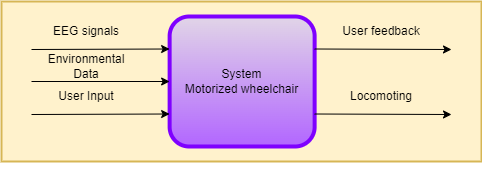
\includegraphics{figs/Level_0_Block_Diagram_Figure_A.2..png}}
        \caption{Level 0 Block Diagram}
        \label{fig:level-0}
    \end{figure}
    \begin{figure}[htbp]
            \centerline{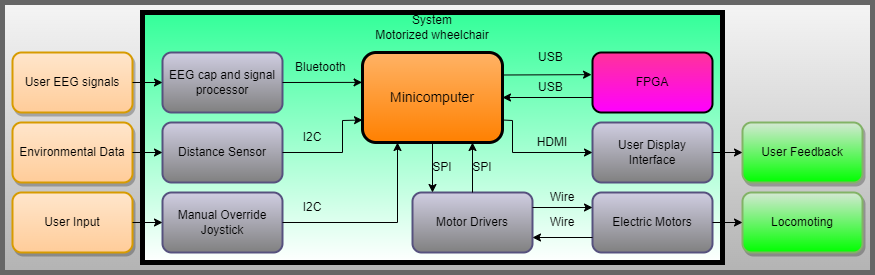
\includegraphics[height=2.4in,keepaspectratio]{figs/Level_1_Diagram_Figure_A.3_2.png}}
            \caption{Level 1 Block Diagram}
            \label{fig:level-1}
        \end{figure}    
    \twocolumn
    %%%%%%%%%%%%%%%%%%%%%%%%%%%%%%%%%%%%%%%%%%%%%%%%%%%%%%%%%%%%%%%%%%%%%%%%%%%%%%%%%%%%%%%%%%%%%%%

\clearpage
\onecolumn
\begin{center}
    \addcontentsline{toc}{section}{Appendix B}
    \vspace*{5cm}
     {\Huge\bfseries Appendix B \par}
     \vspace{1cm}
    \textit{Feasibility Analysis} \\
\end{center}
\clearpage
\twocolumn
\setcounter{section}{2}
\renewcommand{\thesubsection}{B.\Alph{subsection}}

\section*{\textbf{Appendix B}}

    % \renewcommand*{\subsection}
    \setcounter{subsection}{0}
    % \subsection{Feasibility Analysis}
        \subsection{Technological Feasibility}
        The technological feasibility of this project will heavily rely on the team's ability to develop a machine learning model that can interpret brain signals from the EEG cap and translate that into motion controls. The team has found several papers that have done such a thing \cite{robotic_architecture, learning_to_control, toward_brain_computer, self_paced, fpga_intel} so this aspect of the technical feasibility has been deemed feasible. The machine learning process will start in Python to test and train different models. This model will then be translated to C or C++ manually. If sufficient progress has been made, the model will be implemented onto an FPGA either manually or through use of a high level language synthesizer (HIS). This will translate the C or C++ code to an HDL language. While the team has not found anyone else doing this machine learning model implementation for a brain-controlled wheelchair specifically, documentation is available of models being translated to FPGA \cite{fpga_intel}.  

        Next in analyzing the technological feasibility is the motorized wheel chair. Motorized wheelchairs are commercially available for purchase; this aspect of the project is highly feasible. The team will build a motorized wheelchair purely for testing purposes to serve as a proof of concept or prototype.

        \subsection{Time Feasibility}
        The team has created a Gantt Chart, shown in Figure \ref{fig:gantt}, to determine the time feasibility of the project. The Gantt chart will keep us on task and ensure progress is kept on time. This chart shows goals for a time period and how long we have to complete them in an orderly manner. Through delegation of tasks, the team believes that this project is feasible with the time constraints. Kaleb Guillot is prioritizing his software contribution and Gerhort Alford is prioritizing his contributions to designing and implementing the hardware, with crossover in between where needed. The summer months may also be taken advantage of to continue to work on the project and problem-solve. 

        \subsection{Cost Feasibility}
        After arranging a rough bill of materials and taking into account some alternatives the team has concluded that the project will be well within the original budget of \$7,550.00. The rough bill of materials comes out to be {\$4,789.34}, which includes alternatives of the second most expensive parts which are the processors. Even though parts may change, the team is fairly certain that the initial budget will not be exceeded. The team has also been told by the project mentor and sponsor Dr. Magdy Bayoumi that the purchase of a data set for the machine learning model may also be required. He has specifically instructed us to contact him if this situation arises. With this, the cost feasibility of this project is feasible. The rough bill of materials can be seen in Fig. \ref{fig:bom}. 

        \setcounter{figure}{0}
        \renewcommand{\thefigure}{B.\arabic{figure}}
        \begin{figure}
        \centering
        \centerline{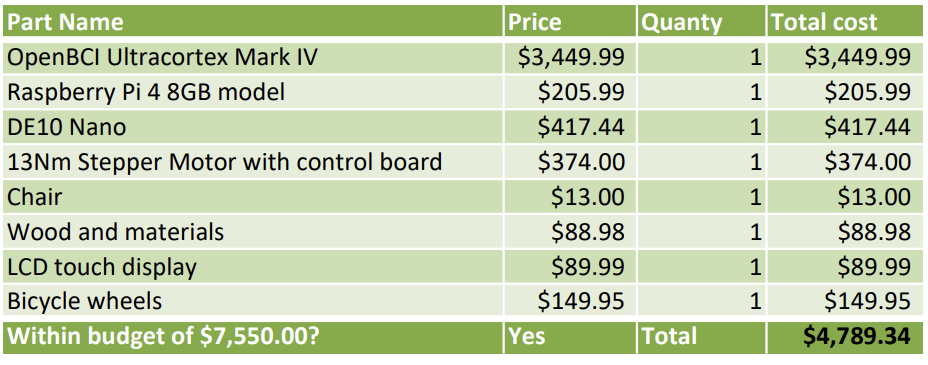
\includegraphics[height=1.35in, keepaspectratio]{figs/BOM.png}}
            \caption{Bill of Materials}
            \label{fig:bom}
            % cite with: s shown in Fig.~\ref{fig:level-0-block-diagram}, the 
        \end{figure}

        \subsection{Legal Consideration}
        Since this project is a prototype and not a final product marketed for public use, there is not worry about legal issues. If this was the final product, the team would have to follow the guide lines for the Food and Drug Administration (FDA) along with American with Disabilities act (ADA) in ensuring the wheelchair is safe and easy to use.

    \clearpage
    \onecolumn
    
    \begin{figure}
        \centering
        \centerline{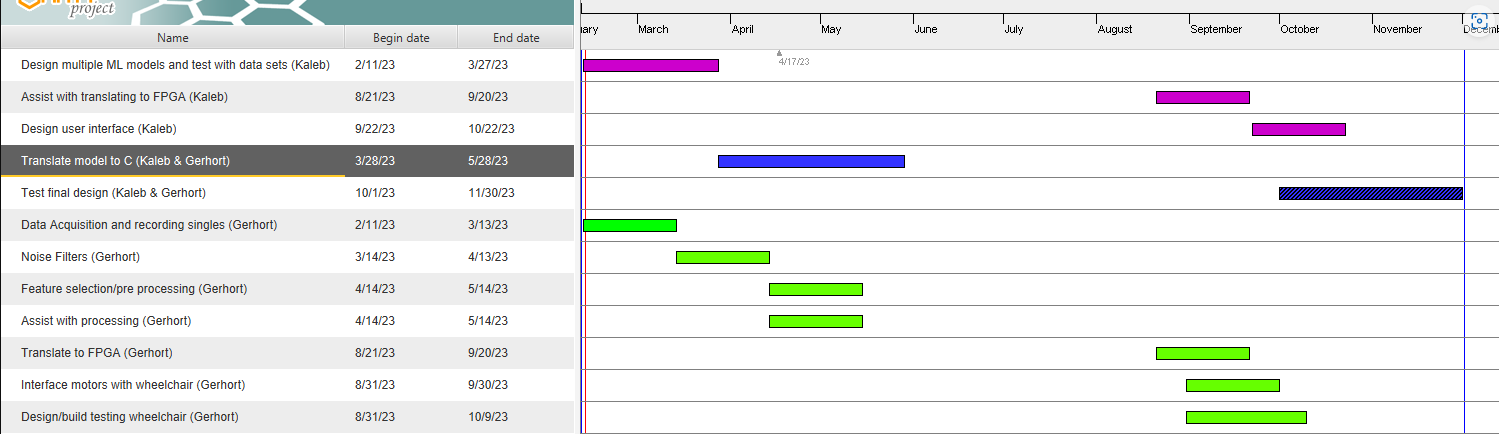
\includegraphics[angle=90, height=9in, keepaspectratio]{figs/gnatt.png}}
            \caption{Gantt Chart}
            \label{fig:gantt}
            % cite with: s shown in Fig.~\ref{fig:level-0-block-diagram}, the 
    \end{figure}
    \twocolumn
    
        
        
\clearpage
\onecolumn
\begin{center}
    \addcontentsline{toc}{section}{Appendix C}
    \vspace*{5cm}
     {\Huge\bfseries Appendix C \par}
     \vspace{1cm}
    \textit{Alternatives and Trade-offs} \\
\end{center}
\clearpage
\twocolumn

\clearpage
\setcounter{section}{3}
\renewcommand{\thesubsection}{C.\Alph{subsection}}
\section*{\textbf{Appendix C}}
        \setcounter{figure}{0}
        \renewcommand{\thefigure}{C.\arabic{figure}}
        \setcounter{table}{0}
        \renewcommand{\thetable}{C.\arabic{table}}
    \setcounter{subsection}{0}
    For both the software and hardware aspects of this project, there are many different, equally feasible paths that can be taken. The team has carefully considered each option and presents the current findings.
    
        \subsection{EEG Caps}
        Based on recommendations by peers and individual research, there are two companies for consideration that sell headsets which were previously used in related projects. These two companies are OpenBCI and G.Tec. OpenBCI is the more widely known of the two, selling caps which allow for full customization and having open-source software libraries beneficial for processing EEG signals. {OpenBCI's Ultracortex Mark IV is being considered by the group due to it having an adequate number of electrodes, an ability to be reassembled with 3-D printed parts, and an ability to work with any of OpenBCI's other microcontrollers.} G.Tec's headsets can be customized even further than what is possible with OpenBCI. G.Tec are the headsets of choice for experts in the field, such as that of \cite{learning_to_control}.  {Of G.Tec's selection, the team found the g.Nautilus Research headset to be suitable for this project due to its electrode placements and comparative affordability to G.Tec's other headsets.} However, due to the complexity and price tag of G.Tec headsets, the team has opted for an OpenBCI headset.
        
        As shown by Table \ref{tab:headsets}, there is one more company, EMOTIV, that sells a plug-and-play headset. Emotiv headsets are suitable for beginners in the field, such as students studying neuroscience. This headset is very high level and does not allow users to access the raw EEG data without a specialized license. The goal of this headset is to merely collect data, not manipulate it. Therefore, it is not suitable for this project in particular, nor does the team believe it suitable for any similar engineering and design work. This claim is backed by the work done in \cite{self_paced, biomedical-signal}. However, the software suite available for this headset is very eye-catching, allowing users to move virtual objects based on pre-designed models. The  {EMOTIV EPOC X} headset is available for the team's use, purchased by the mentor and sponsor. For these reasons, the team is developing an attraction using this headset for E\&T Week. 
        
        \subsection{Minicomputers}
        The processing is a critically important part of this project as it employs a pre-trained machine learning model, interpreting the brain signals from the EEG cap. This requires several powerful, portable processing units and pieces of hardware. Table \ref{tab:minicomputer} presents the current findings. The team is considering several minicomputers, weighing the power of their CPU, availability of peripherals, available documentation, and accessibility. The three currently in consideration are the Jetson nano, Orange Pi 5, and Raspberry Pi 4. The team's processing needs are similar to that of image processing; the incoming signals from the EEG cap will be treated like an image and will be compared to the movement signals. This process needs to be as fast as possible, so when the user of the wheelchair wants to move forward they can move nearly instantaneously. These minicomputers, however, are not powerful enough to process a robust model in an efficient manner. The processors will need to be supplemented with another piece of hardware, such as an FPGA, that will handle the simple, repetitive calculations. 
        
        With these factors in mind, the team has carefully weighed the options based on recommendations by peers and independent research. The first option was the popular Raspberry Pi 4, with the pull of a wealth of documentation. This processor, however, is currently hard to obtain due to shortages, leading us to the Orange Pi 5. The Orange Pi 5 is akin to the Raspberry, but with the addition of built in tensor processing capabilities with an ARM Mali-G610 MP4 GPU. The final option is the Jetson Nano. The Nano is powerful enough to run Ubuntu, and only comes in at a slightly higher price than the Orange Pi 5. However, due to the ease of use and increased RAM of the Orange Pi 5, it is a front runner.
        
        \subsection{Motors}
        On the wheelchair, two motors will be employed to drive two of the wheels of the wheelchair. The motors will be responsible for receiving the signal from the processing unit and outputting accurate and reliable movement. This requires motors that are capable of producing high torque at slow speeds. The position of the motor needs to be known, keeping tabs on the traction of the wheels and having the ability to know the actual speed compared to the outputted, desired speed. This can allow for adjustments and calibrations to be made automatically. 
        
         {There are three types of motors under consideration. They are servo, stepper, and DC motor with a worm drive.} These motors are displayed in Table \ref{tab:motors}.  {The team has decided to use a DC motor with a worm drive. This type of motor consists of a brushed DC motor that drives a reduction worm gear. In a worm gear system, a screw-like gear drives a helical gear at a much slower speed, but with significantly higher torque than the motor shaft. The team has chosen this option for three main reasons. Firstly, the worm drive significantly reduces the motor's revolutions per minute while increasing its torque output, which is ideal for the slow speed requirements of a wheelchair. Secondly, the worm gear system makes it difficult to turn the output shaft, which is beneficial for ensuring that the wheelchair remains stationary if the power supply fails. Finally, the cost of this option is the most affordable, even with the added expense of the necessary hardware for feedback.} 

        \subsection{FPGAs}
        There are two main FPGA manufacturers: Xilinx which is owned by AMD and Altera which is owned by Intel. The analysis of the alternatives and tradeoffs for these two manufacturers are shown in Table \ref{tab:fpga}. There are many different boards these manufacturers make, each with similar capabilities for the purposes of this project. While Intel has a larger selection, Xilinx is the current favorite due to the ability to coincide with the other components of the design. The main concern for the project is the integrated synthesis environment (ISE) both these manufacturers use. Both can be downloaded and used for free, so price is not a concern. These ISEs will be able to translate the machine learning model in C++ to VHDL, Verilog, or System Verilog. Since the team has access to boards from both manufacturers, it will be easy to test which ISE is better at converting the machine learning model to a hardware description language like Verilog, System Verilog, or VHDL. From each of these manufacturers, the two boards the team has held in consideration are the Xilinx TUL PYNQ-Z2 and the Altera DE10-Nano. Both have similar hardware available, however the  {group has elected to use the Xilinx TUL PYNQ-Z2}  due to its ease of use and the ability to interface with external minicomputers. 

        \subsection{Environmental Sensors}
            \subsubsection{Distance Sensors}
            For the wheelchair to gather information about the surrounding environment, sensors that measure distance must be used to detect any potential obstacles. The sensors that were considered by the team are shown in Table \ref{tab:sensors}. They include ultrasonic, infrared, LIDAR, and cameras. 
            
            Ultrasonic sensors emit high-frequency sound waves that detect the reflected sound to calculate distance. These sensors are cheap and have a wide field of view, however they are susceptible to interference, have limited resolution, and have limited accuracy. 
    
            Infrared sensors detect the presence of obstacles through emitting infrared radiation and then calculating the reflected radiation. They are cheap, have good range, and are suitable for indoor use, which is beneficial for a wheelchair that will likely spend a considerable amount of time indoors. However, infrared sensors have a limited field of view, are affected by temperature, and have limited accuracy.
    
            LIDAR sensors use light to detect the distance and location of objects in the environment. These sensors are often used on similar projects \cite{learning_to_control, openbci-research, collab_controller} as they are accurate, have a long range, are capable of 3-D mapping, and are resistant to environmental interference. It comes as no surprise that the disadvantages of these sensors are their cost and required processing power.
    
            Cameras are another popular choice for similar projects \cite{learning_to_control, openbci-research}. Cameras are a similar story to LIDAR, as they have many of the same capabilities with the additional ability to distinguish color and process images. The disadvantages are similar as well, as cameras require high processing power, high cost, and high overhead. 
    
            After careful consideration, the team has elected to use a combination of ultrasonic and infrared sensors. These sensors have low form factors, are lightweight, and are low-cost. They function well at similar ranges, with ultrasonic sensors working well with hard surfaces and infrared sensors working well with reflective surfaces. They will work to compensate for the limitations of each other, as each sensor's functionality declines in different environments. 

            \subsubsection{ {Inertial Measurement Units}}
            Information about the wheelchair's orientation and acceleration can prove to be key safety features when interfaced with the motor drivers and braking system. These sensors will also provide another layer of feedback to the ensure that the outputted commands sent to the motor drivers are adequately performed by the motors. The analysis of different types of inertial measurement units (IMUs) are shown in Table \ref{tab:imu}, referencing three types of units. They are the micro-electro-mechanical system (MEMS) IMU, fiber optic gyro (FOG) IMU, and the ring laser gyro (RLG) IMU. This subsection will explore the key differences between these three IMUs.

            The MEMS IMU is best known for its applications in mobile devices, such as smart phones and smart watches. To take measurements of acceleration and rotation, they utilize tiny mechanical structures that make the MEMS lightweight and affordable. The accuracy of these IMUs is normally inferior to other types of IMUs, as they are susceptible to noise and other sources of error. While these IMUs require precise calibration and filtering, they are typically easily integrated with other sensors and electronics, making them suitable for this project.

            The FOG IMU uses fiber optics to detect changes in the orientation of a system. They consist of a coil of optical fiber that is wound around a rotating spindle. The measurements are recorded through the roation of the spindle which causes the light passing through the fiber to experience a phase shift. FOG IMUs are often used in applications where accuracy and precision are quintessential, such as in aerospace and robotics. They are very reliable, offering continuous measurement of rotation rates and high accuracy, even in harsh conditions. These IMUs are more expensive, have a larger form factor, and require additional measures to maintain stability over time. Due to high priority of safety of this project, these sensors would be beneficial to include.

            The RLG IMU use ring laser gyros to measure rotation. They consist of a closed loop of laser light that is split into two beams traveling in opposite directions. When the loop rotates, it causes a phase shift in the two beams, capturing the rotation. They are akin to the FOG IMU in their reliability, accuracy, need for additional measures to maintain stability, and high price. They excel compared to FOG IMUs in their compact and lightweight design, and far exceed MEMS IMUs in their continuous measurements and stability over time. For a commercial application of this project, these sensors would be beneficial to include.  

            After consideration, the group has opted for the MEMs IMU due to its adequate accuracy and reliability, and it being more affordable and easy to work with compared to the RLG and FOG IMUs.

        \subsection{ {Software}}
            \subsubsection{Machine Learning}
            In order to correctly classify the user's intent while wearing the EEG cap, a machine learning model must be trained. This model needs to classify input from the EEG cap and environmental sensors quickly and effectively, while remaining simplistic enough to fit on the onboard minicomputer. There are four models that the team is considering: Random Forest, Convolutional Neural Network (CNN), Long Short-Term Memory (LSTM), and Gated Recurrent Unit (GRU). 
            
            A Random Forest is a type of ensemble learning algorithm that combines multiple decision trees to make predictions. This means that multiple algorithms will be combined in order to make a final prediction. This is the most robust of the options, as a Random Forest can encapsulate one or more of the other models under consideration. A CNN is a very popular model often used for classifying images by performing convolutional calculations on subsets of the pixels in the image. This model is the most simple of the ones under consideration and has the downside of not capturing the temporal locality of predictions. An LSTM is a type of Recurrent Neural Network (RNN) that captures temporal locality through its ability to handle long-term dependencies in sequential data. A single LSTM block contains three main components: an input gate, output gate, and a forget gate. This model is very popular and robust, making accurate predictions but requiring powerful hardware to run efficiently. A GRU is similar to an LSTM in capturing temporal locality, however it is computationally more simple. These networks only have two gates: an update gate and a reset gate. 
            
            These options are displayed in Table \ref{tab:ml-tbl}, showing a brief description, the pros and cons, and a rationale of the team's choice. The team has opted to use a CNN to classify the EEG and sensor data, as the team is familiar with this model and believes it be sufficient for use in this project.
        \onecolumn
        \renewcommand{\arraystretch}{3}
        \setlength{\arrayrulewidth}{1.5pt}

        \begin{table}[htbp]
            \centering
            \begin{tabular}{|>{\raggedright\arraybackslash}c|>{\raggedright\arraybackslash}p{0.25\linewidth}|>{\columncolor{orange!20}\raggedright\arraybackslash}p{0.25\linewidth}|>{\raggedright\arraybackslash}p{0.25\linewidth}|}
                \hline
                \textbf{\textit{EEG Caps}} & \textbf{EMOTIV EPOC X} & \textbf{Ultracortex Mark IV} & \textbf{g.NAUTILUS} \\
                \hline

                \rule{0pt}{4cm}\multirow{-3}{*}{\textit{Picture}} & \adjustbox{center}{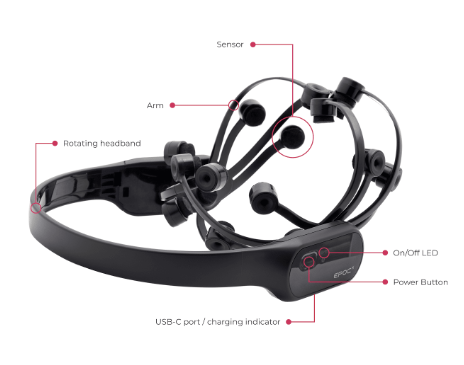
\includegraphics[height=1.3in,keepaspectratio]{figs/alts-pics/emotiv.png}} & \centering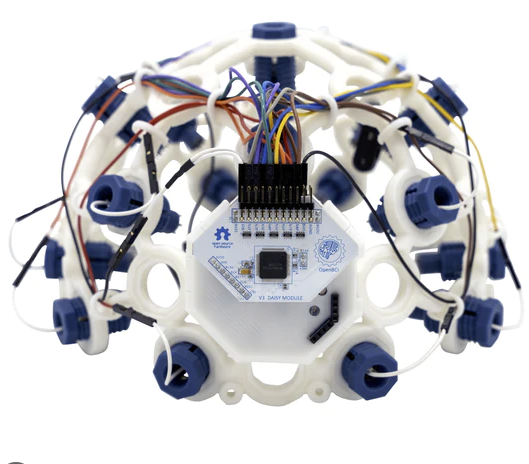
\includegraphics[height=1.3in, keepaspectratio]{figs/alts-pics/ultracortex.png} & \adjustbox{center}{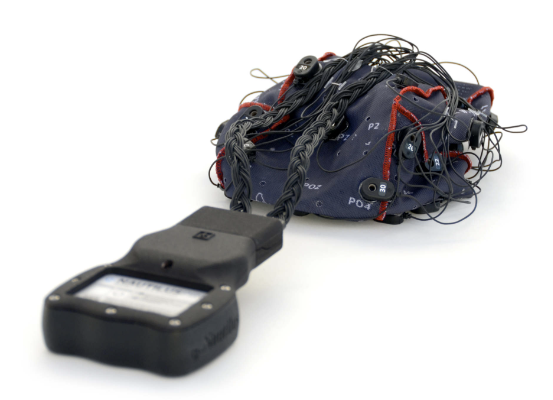
\includegraphics[height=1.3in, keepaspectratio]{figs/alts-pics/g-tec.png}}
                
                \\
                
                \textit{Description and Specs} & Lightweight EEG cap with 14 channels & Highly customizable 16 channel EEG cap & Professional grade 4-64 channel EEG cap \\ 

                \hline

                \multirow{3}{*}{\textit{Pros}} & \begin{itemize}
                                    \item Beginner friendly software
                                    \item Has 5 trainable models to use, no machine learning required
                                    \item Available APIs for customized applications
                                \end{itemize}
                            &  \begin{itemize}
                                \item Very customizable and easy to make modifications
                                    \item Good documentation and software libraries available in many programming languages
                                \end{itemize}
                            & \begin{itemize}
                                \item Professional build quality
                                \item Highly customizable
                                \item Available Software libraries and APIs
                            \end{itemize}
                            \\

                \multirow{3}{*}{\textit{Cons}} & \begin{itemize}
                                    \item Fragile
                                    \item Access to raw EEG data is locked behind paywall
                                    \item Must be connected to wifi at all times
                                    \item Electrodes must be constantly adjusted
                                \end{itemize}

                            & \begin{itemize}
                                    \item Some self-assembly required
                                    \item Cheap, 3D printed build quality
                                \end{itemize}

                            & \begin{itemize}
                                    \item Very expensive
                                    \item Requires extensive knowledge of the field for proper use
                                \end{itemize}
                                \\
                \multirow{2}{*}{\textit{Rationale}} & EMOTIV headsets are not intended to be used for technological research 
                & OpenBCI has a wealth of software and hardware tools available and its intended use is for technological research
                & Out of price range \\
                \hline
            \end{tabular}
            % \captionsetup{skip=10pt}
            \caption{EEG Headset Alternatives and Tradeoffs}
            \label{tab:headsets}
        \end{table}

        \begin{table}[htbp]
            \centering
            \begin{tabular}{|>{\raggedright\arraybackslash}c|>{\raggedright\arraybackslash}p{0.25\linewidth}|>{\columncolor{orange!20}\raggedright\arraybackslash}p{0.25\linewidth}|>{\raggedright\arraybackslash}p{0.25\linewidth}|}
            \hline
            \textbf{\textit{Minicomputers}} & \textbf{Raspberry Pi 4} & \textbf{Orange Pi 5} & \textbf{Jetson Nano} \\
            \hline
            \rule{0pt}{4cm}\multirow{-3}{*}{\textit{Picture}} 
                & \centering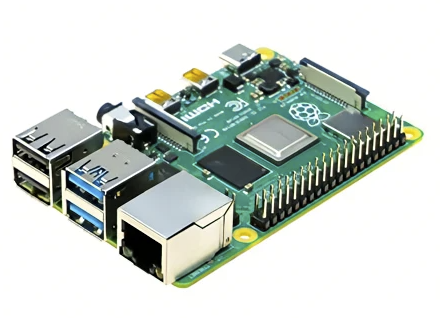
\includegraphics[height=1.3in,keepaspectratio]{figs/alts-pics/raspberry.png}& \centering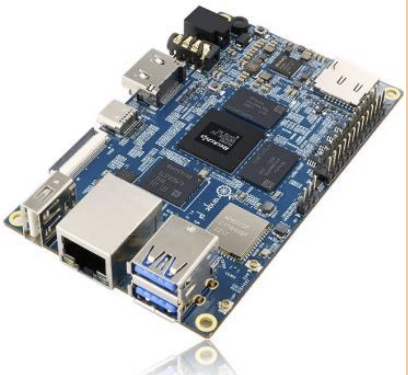
\includegraphics[height=1.3in,keepaspectratio]{figs/alts-pics/orange.png} & \adjustbox{center}{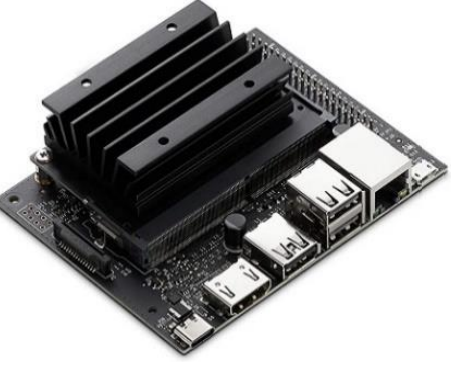
\includegraphics[height=1.3in,keepaspectratio]{figs/alts-pics/jetson.png}} \\

            \multirow{6}{*}{\textit{Description and Specs}} & Minicomputer that runs a Debian Linux based operating system \begin{itemize}
                                \item CPU: Quad core Cortex-A72 (ARM v8) 64-bit SoC @ 1.8GHz
                                \item RAM: 1-8 GB SDRAM
                                \item 1 x USB C port
                                \item 2 x micro HDMI ports
                                \item 2 x USB 3.0 ports
                                \item 2 x USB 2.0 ports
                                \item 2-lane MIPI DSI display port
                                \item Gigaabit Ethernet port
                                \item 2.4GHz and 5.0 GHz IEEE 
                                \item 802.11ac wireless
                                \item Bluetooth 5.0
                                \item 26 GPIO headers
                            \end{itemize}
                        & Minicomputer that runs Android based operating system
                        \begin{itemize}
                            \item CPU: Rockchip RK3588S octa-core 64-bit processor, Main frequency up to 2.4GHz
                            \item RAM size: 4-32GB LPDDR4
                            \item GPU: Arm Mali-G610 MP4
                            \item NPU: Built-in AI accelerator NPU with up to 6 TOPS, supports INT4/INT8/INT16 mixed operation
                            \item PMU: RK806-1
                            \item Micro-SD card slot
                            \item 1 x HDMI 2.1 port
                            \item 2 x USB 3.0 port
                            \item 1 x USB 2.0 port
                            \item 1 x Ethernet port
                            \item M.2 M-KEY Socket
                            \item 26 GPIO headers
                        \end{itemize}
                        
                        & Minicomputer that runs OS based on Ubuntu 10.04 (Linux4Tegra)
                        \begin{itemize}
                            \item CPU: Quad-core ARM Cortex-A57 
                            \item MPCore processor
                            \item RAM size: 4 GB 64-bit LPDDR4
                            \item 16GB eMMC5.1
                            \item 2 x USB 3.0
                            \item 1 x USB 2.0
                            \item 1 x HDMI 2.0
                            \item 1 x USB Micro-B
                            \item 26 GPIO pins
                            \item M.2 Key E slot
                        \end{itemize}
                        
                        \\ 
            \hline
            \textit{Cost} & \$75.00-\$205.00 & \$130.00 & \$149.00 \\

            \multirow{3}{*}{\textit{Pros}} & \begin{itemize}
                                \item Good documentation
                                \item Built in WiFi and Bluetooth
                                \item 4 USB Ports
                            \end{itemize}
                        & \begin{itemize}
                            \item Good availability
                            \item Hardware capable of machine learning
                            \item Most powerful CPU
                        \end{itemize}
                        
                        & \begin{itemize}
                            \item Good availability
                            \item Hardware capable of machine learning
                            \item Most powerful GPU
                        \end{itemize}
                        \\
            \multirow{3}{*}{\textit{Cons}} 
                & 
                \begin{itemize}
                    \item Shortages; hard to obtain
                    \item Need external hardware to perform machine learning
                \end{itemize}
                & 
                \begin{itemize}
                    \item New product, not well documented
                    \item No built in WiFi or Bluetooth
                \end{itemize}
                & 
                \begin{itemize}
                    \item Not well documented
                \end{itemize}
                \\
            \multirow{2}{*}{\textit{Rationale}} 
                & Not capable of running machine learning algorithm on its own
                & Hardware is capable of performing machine learning. Available to the group. 
                & Not available to the group \\
            \hline
            \end{tabular}
            \caption{Minicomputer Alternatives and Tradeoffs}
            \label{tab:minicomputer}
            
        \end{table}

        \begin{table}[htbp]
            \centering
            \begin{tabular}{|>{\raggedright\arraybackslash}c|>{\raggedright\arraybackslash}p{0.25\linewidth}|>{\raggedright\arraybackslash}p{0.25\linewidth}|>{\columncolor{orange!20}\raggedright\arraybackslash}p{0.25\linewidth}|}
            \hline
                 \textbf{\textit{Motor Type}} & \textbf{Servo} & \textbf{Stepper} & \textbf{DC Motor with Worm Drive}  \\
            \hline
                 \rule{0pt}{4cm}\multirow{-4}{*}{\textit{Picture}} & \centering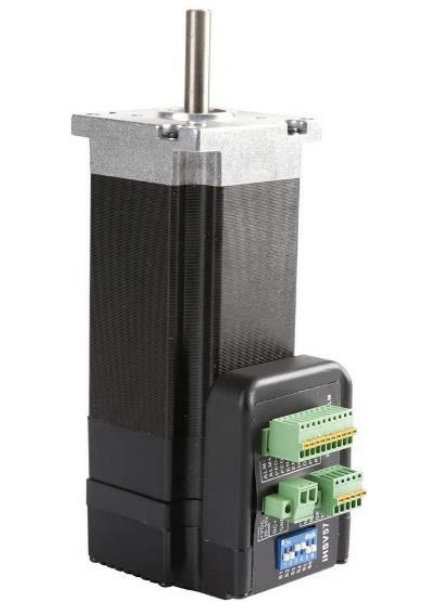
\includegraphics[height=1.5in, keepaspectratio]{figs/alts-pics/servo.png} & \adjustbox{center}{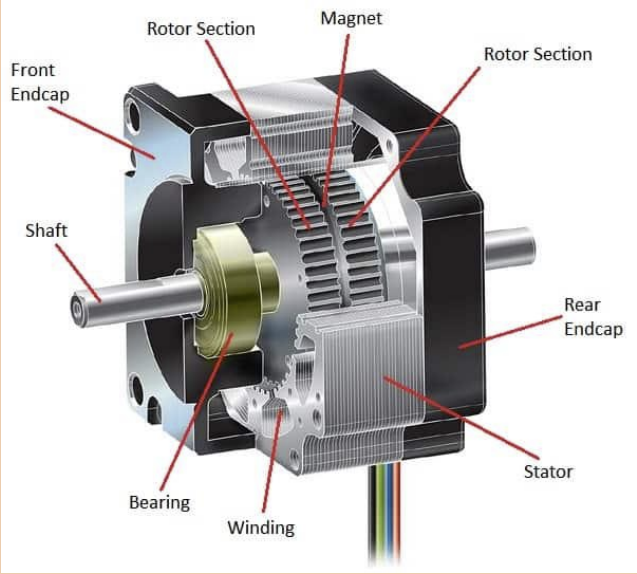
\includegraphics[height=1.5in, keepaspectratio]{figs/alts-pics/stepper.png}} & \adjustbox{center}{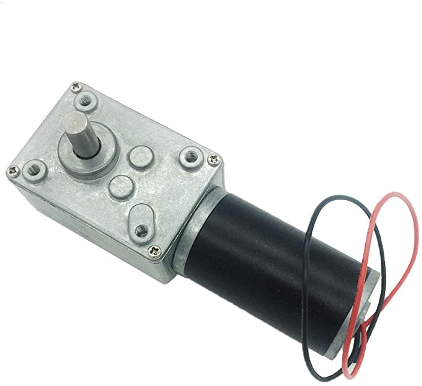
\includegraphics[height=1.5in, keepaspectratio]{figs/alts-pics/worm_drive.png}}\\

                \multirow{1}{*}{\textit{Description and Specs}} 
                & Use radially magnetized rotors to turn 
                & Motor rotation is controlled by an electric pulse
                & Brushed DC motor with a worm drive reduction gear \\
            \hline
                \textit{Cost Range} & \$100.00 - \$400.00 & \$85.00 - \$200.00 & \$12.00 - \$60.00 \\
                \multirow{2}{*}{\textit{Pros}} 
                & 
                \begin{itemize}
                    \item Closed loop feedback
                    \item High torque at high speeds
                \end{itemize}
                & 
                \begin{itemize}
                    \item High torque at low speeds
                    \item Lower cost
                    \item Quick response
                    \item Smaller form factor
                \end{itemize}
                &
                \begin{itemize}
                    \item High torque at low speeds
                    \item Lowest cost
                    \item Will not turn without power. Wheelchair will stay in place if power is lost
                \end{itemize}
                \\
            \multirow{3}{*}{\textit{Cons}} 
                &
                \begin{itemize}
                    \item Slow response
                    \item Longer body
                    \item Higher Cost
                    \item Low torque at low speeds
                \end{itemize}
                &
                \begin{itemize}
                    \item No feedback; needed for this project's design needs
                    \item Lower torque at high speeds
                \end{itemize}            &
                \begin{itemize}
                    \item Need to add feedback for wheelchair, requires extra components
                    \item Many of these motors are only capable of low speeds due to gear reduction. 
                \end{itemize}
                \\
            \multirow{1}{*}{\textit{Rationale}} 
                & External braking mechanism would be needed. Does not automatically brake without
                & Spins freely without power 
                & Automatically brakes when no power is supplied. Low speed with high torque.  \\
            \hline
                 
            \end{tabular}
            \caption{Motor Alternatives and Tradeoffs}
            \label{tab:motors}
        \end{table}

        \begin{table}[htbp]
            \centering
            \begin{tabular}{|c|>{\columncolor{orange!20}\raggedright\arraybackslash}p{0.4\linewidth}|>{\raggedright\arraybackslash}p{0.4\linewidth}|}
            \hline
                 \textbf{\textit{FPGAs}} & \textbf{TUL PYNQ-Z2} & \textbf{DE10-Nano}  \\
            \hline
                 \rule{0pt}{4.5cm}\multirow{-4}{*}{\textit{Picture}} & \adjustbox{center}{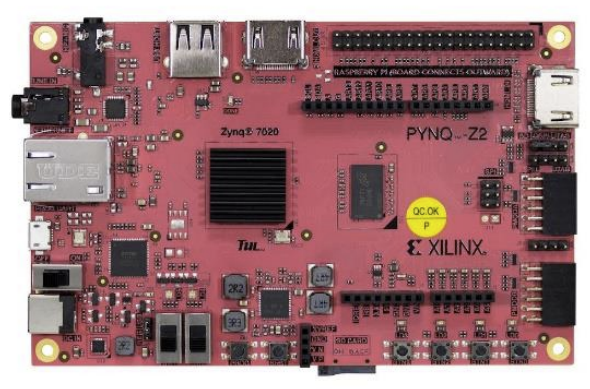
\includegraphics[height=1.5in, keepaspectratio]{figs/alts-pics/tulpynq.png}} & \adjustbox{center}{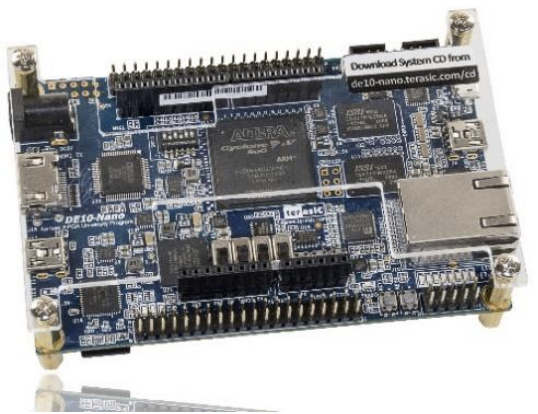
\includegraphics[height=1.5in, keepaspectratio]{figs/alts-pics/de10.png}}
                 \\

                \multirow{3}{*}{\textit{Description and Specs}} 
                &
                Xilinx FPGA with a dual core ARM cortex A9 processor. 
                \begin{itemize}
                    \item 85K logic cells (13300 logic slices, each with four 6-input LUTs and 8 flip-flops)
                    \item 220 DSP slices
                    \item 630 KB of fast block RAM
                \end{itemize}
                &
                Altera FPGA with a dual core ARM cortex A9 processor.
                \begin{itemize}
                    \item Logic elements (LE): 110 K LE
                    \item 5,570 kilobits memory
                    \item 224 18 x 19 multipliers
                    \item 112 variable precision DSP blocks
                    \item 6 phased-locked loops (PLL)
                    \item 145 user-defined I/O
                \end{itemize}
                \\
            \hline
                \textit{Cost Range} & \$123.00 & \$417.44 \\
                \multirow{3}{*}{\textit{Pros}} 
                &
                \begin{itemize}
                    \item Can run programs written in Python
                    \item Lower Price
                    \item Has Raspberry Pi style 26 pin GPIO headers
                    \item Developer tools can be used for free
                \end{itemize}
                & 
                \begin{itemize}
                    \item In stock
                    \item Large user community with copious amount of documentation
                    \item Many connections for peripherals
                \end{itemize}\\
                \multirow{2}{*}{\textit{Cons}} 
                &
                \begin{itemize}
                    \item Not as much documentation
                    \item Hard to find
                \end{itemize}
                &
                \begin{itemize}
                    \item Expensive
                    \item Does not support Python
                    \item Developer tools are limited
                \end{itemize}
                \\
            \multirow{1}{*}{\textit{Rationale}}
                & Compatible with the chosen minicomputer and much simpler to work with.
                & Lower level and much more difficult to work with. \\ 
            \hline
                 
            \end{tabular}
            \caption{FPGA Alternatives and Tradeoffs}
            \label{tab:fpga}
        \end{table}
        
        \begin{table}[htbp]
            \centering
            \begin{tabular}{|c|>{\columncolor{orange!20}\raggedright\arraybackslash}p{0.18\linewidth}|>{\columncolor{orange!20}\raggedright\arraybackslash}p{0.18\linewidth}|>{\raggedright\arraybackslash}p{0.18\linewidth}|>{\raggedright\arraybackslash}p{0.18\linewidth}|}
            \hline
                 \textbf{\textit{Sensor}} & \textbf{Ultrasonic} & \textbf{Infrared} & \textbf{LIDAR} & \textbf{Camera}  \\
            \hline
                 \rule{0pt}{3cm}\multirow{-3}{*}{\textit{Picture}} & \adjustbox{center}{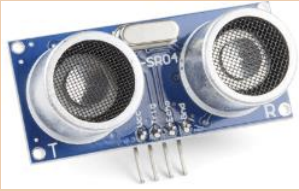
\includegraphics[height=1in, width=1.3in]{figs/alts-pics/ultrasonic.png}}& \adjustbox{center}{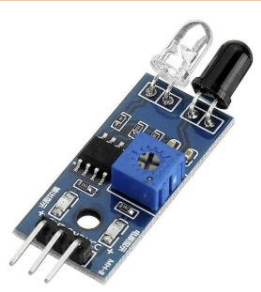
\includegraphics[height=1in]{figs/alts-pics/infrared.png}} & \adjustbox{center}{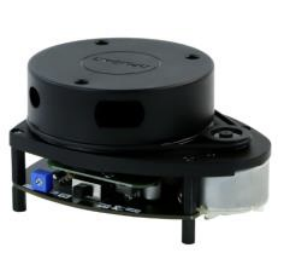
\includegraphics[height=1in]{figs/alts-pics/lidar.png}} & \adjustbox{center}{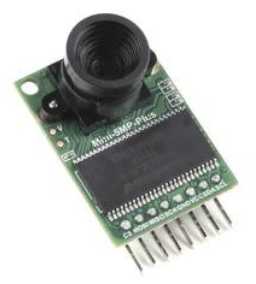
\includegraphics[height=1in]{figs/alts-pics/camera.png}}\\

                \multirow{2}{*}{\textit{Description and Specs}} & Emits high frequency sound waves that detect the reflected sound & Emits infrared radiation and then detects the reflected signal & Emits laser light and detects the reflected signal & Captures and records light that enters the lens \\
            \hline
                \textit{Cost Range} & \$3.75 - \$34.95 & \$3.95 - \$26.75 & \$25.99 - \$999.00 & \$59.99 - \$800.00 \\
                \multirow{2}{*}{\textit{Pros}} 
                &
                \begin{itemize}
                    \item Affordable
                    \item Wide field of view
                \end{itemize}
                & 
                \begin{itemize}
                    \item Affordable
                    \item Suitable for indoor use
                \end{itemize}
                &
                \begin{itemize}
                    \item Accurate
                    \item Long range
                    \item 3D mapping
                    \item Resilient
                \end{itemize}
                & 
                \begin{itemize}
                    \item Accurate
                    \item Object Detection
                \end{itemize}
                \\
                \multirow{2}{*}{\textit{Cons}} 
                & 
                \begin{itemize}
                    \item Susceptible to interface
                    \item Limited resolution
                    \item Limited accuracy
                \end{itemize}
                & 
                \begin{itemize}
                    \item Limited field of view
                    \item Affected by temperature
                    \item Limited accuracy
                \end{itemize}
                & 
                \begin{itemize}
                    \item High cost
                    \item High processing power
                    \item High overhead
                \end{itemize}
                & 
                \begin{itemize}
                    \item High cost
                    \item High processing power
                    \item High overhead
                \end{itemize}
                \\
            \multirow{1}{*}{\textit{Rationale}}
                & Simple, effective, easy to work with
                & Simple, effective, easy to work with
                & Complex, requires a lot of software overhead, and  expensive.
                & Complex and requires a lot of software overhead
                \\
            \hline
                 
            \end{tabular}
            \caption{Environmental Sensor Alternatives and Tradeoffs}
            \label{tab:sensors}
        \end{table}
        
        \begin{table}[htbp]
            \centering
            \begin{tabular}{|>{\raggedright\arraybackslash}c|>{\columncolor{orange!20}\raggedright\arraybackslash}p{0.25\linewidth}|>{\raggedright\arraybackslash}p{0.25\linewidth}|>{\raggedright\arraybackslash}p{0.25\linewidth}|}
            \hline
            \textbf{\textit{IMUs}} & \textbf{MEMs} & \textbf{FOG} & \textbf{RLG} \\
            \hline
            \rule{0pt}{4cm}\multirow{-3}{*}{\textit{Picture}} & \centering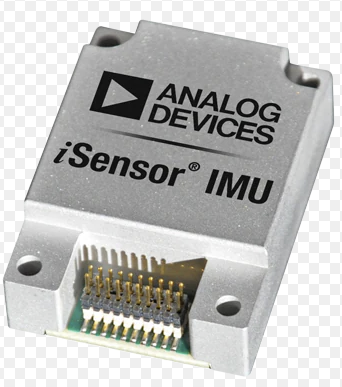
\includegraphics[height=1.3in,keepaspectratio]{figs/alts-pics/mems.png}& \centering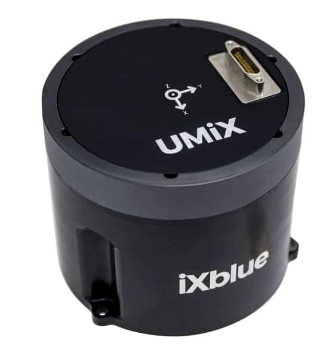
\includegraphics[height=1.3in,keepaspectratio]{figs/alts-pics/fog.png} & \adjustbox{center}{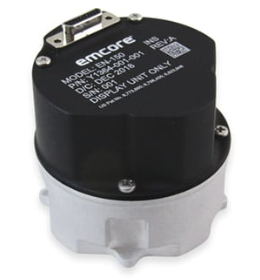
\includegraphics[height=1.3in,keepaspectratio]{figs/alts-pics/rlg.png}}  \\

            \multirow{2}{*}{\textit{Description and Specs}} & Micro-Electro-Mechanical Systems IMUs are small IMUs that use mechanical means to measure acceleration and rotation rates. Commonly used in lightweight applications. 
            & Fiber Optic Gyro IMUs use fiber optics to measure rotation rates. Commonly used in high-end applications
            & Ring Laser Gyro IMUs are similar to FOG IMUs but instead use lasers to measure rates of rotation.
           \\ 
            \hline
            \textit{Cost} & \$10.00-\$200.00 & \$30.00 - \$10,000.00 & \$50.00 - \$100,000.00 \\

            \multirow{3}{*}{\textit{Pros}} & \begin{itemize}
                                \item Most affordable
                                \item Small form factor
                            \end{itemize}
                        & \begin{itemize}
                            \item Very accurate
                            \item Very reliable
                            \item More stable over time than MEMS
                            \item Continuous measurements of rotation rates
                        \end{itemize}
                        
                        & \begin{itemize}
                            \item Very accurate
                            \item Very reliable
                            \item More stable over time than MEMS
                            \item Continuous measurements of rotation rates
                        \end{itemize}
                        \\
            \multirow{3}{*}{\textit{Cons}} 
                & 
                \begin{itemize}
                    \item Cheapest IMUs
                    \item Susceptible to noise and other sources of error
                    \item Require additional calibration
                \end{itemize}
                & 
                \begin{itemize}
                    \item Expensive
                    \item Larger and heavier
                    \item Requires additional cooling and other measures to remain stable
                \end{itemize}
                & 
                \begin{itemize}
                    \item Expensive
                    \item Larger and heavier
                    \item Requires additional cooling and other measures to remain stable
                \end{itemize}
                \\
            \multirow{1}{*}{\textit{Rationale}} 
                & Accurate enough, more affordable, more software libraries available.
                & Accurate, but takes much more time and effort to calibrate. Is also more expensive. 
                & Accurate, but takes much more time and effort to calibrate. Is also more expensive. 
                \\
            \hline
            \end{tabular}
            \caption{IMU Alternatives and Tradeoffs}
            \label{tab:imu}
            
        \end{table}
        
        \begin{table}[htbp]
            \centering
            \begin{tabular}{|c|p{0.18\linewidth}|>{\columncolor{orange!20}\raggedright\arraybackslash}p{0.18\linewidth}|>{\raggedright\arraybackslash}p{0.18\linewidth}|>{\raggedright\arraybackslash}p{0.18\linewidth}|}
            \hline
                 \textbf{\textit{Model}} & \textbf{Random Forest} & \textbf{Convolutional Neural Network (CNN)} & \textbf{Long Short-Term Memory (LSTM)} & \textbf{Gated Recurrent Unit (GRU)}  \\
            \hline
                 \rule{0pt}{3cm}\multirow{-3}{*}{\textit{Picture}} & \adjustbox{center}{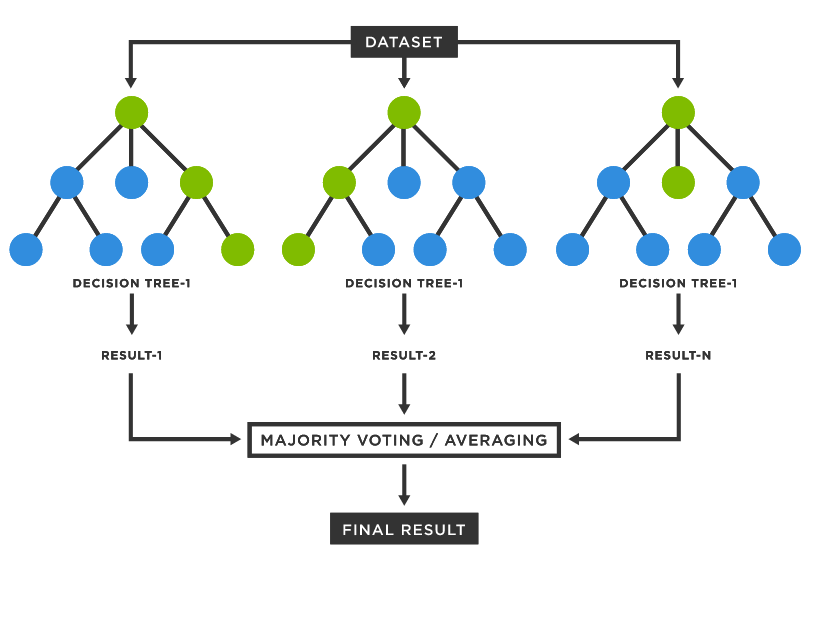
\includegraphics[height=1in, width=1.3in]{figs/alts-pics/random-forest.png}}& \adjustbox{center}{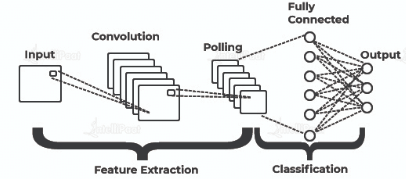
\includegraphics[height=1in, width=1.35in]{figs/alts-pics/cnn2.png}} & \adjustbox{center}{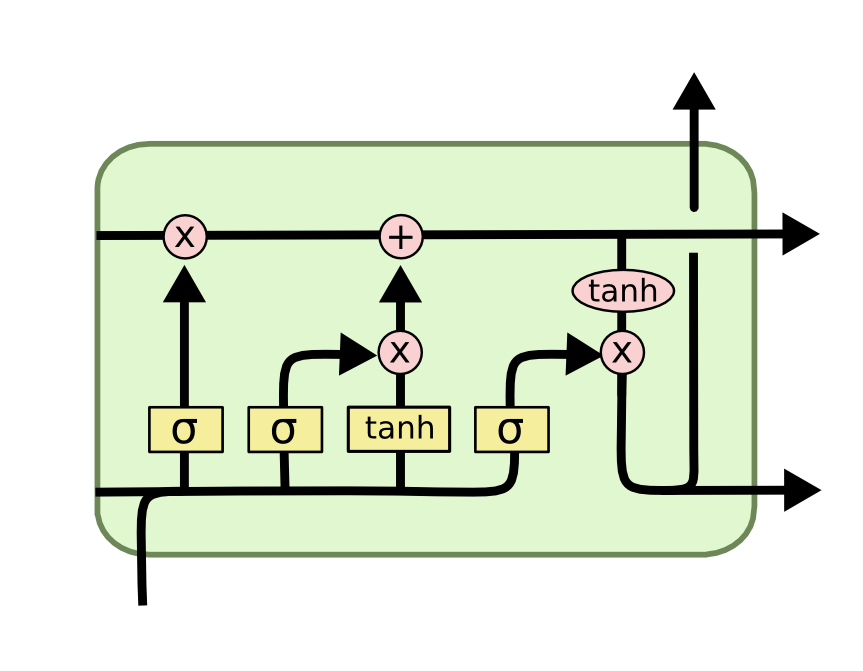
\includegraphics[height=1in]{figs/alts-pics/lstm.png}} & \adjustbox{center}{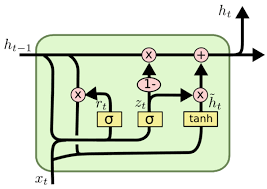
\includegraphics[height=1in]{figs/alts-pics/gru.png}}\\

                \multirow{2}{*}{\textit{Description and Specs}} 
                & An ensemble architecture that makes decisions based on multiple trees by splitting training data between the trees. Consists of a varying number of different architectures and chooses the best one. 
                & An architecture that divides the input data into individual pixels and performs convolutional calculations to find features. The data is subsequently fed into an MLP.
                & An evolution of an RNN that uses and input, output, and forget gate to capture long-term dependencies in input data.
                & An evolution of an RNN that uses an update and reset gate to capture long and short-term dependencies in input data. \\
            \hline

                \multirow{3}{*}{\textit{Pros}} 
                &
                \begin{itemize}
                    \item High accuracy
                    \item High variability
                    \item Most robust model
                \end{itemize}
                & 
                \begin{itemize}
                    \item Most simplistic
                    \item Good historical performance for classification of image data
                \end{itemize}
                &
                \begin{itemize}
                    \item Able to capture long term dependencies
                    \item Able to compare results from previous block and predict following blocks
                \end{itemize}
                & 
                \begin{itemize}
                    \item Able to capture long and short-term dependencies
                    \item Able to compare results from previous block and predict the following blocks
                \end{itemize}
                \\
            \multirow{3}{*}{\textit{Cons}} 
                & 
                \begin{itemize}
                    \item Highest overhead required
                    \item Most complex and computationally intense
                \end{itemize}
                & 
                \begin{itemize}
                    \item Most simplistic
                    \item Still requires a fair amount of computation power
                \end{itemize}
                & 
                \begin{itemize}
                    \item Computationally intense
                    \item Complex
                    \item Has capabilities that may not be required for this application
                \end{itemize}
                & 
                \begin{itemize}
                    \item Computationally intense
                    \item Complex
                    \item Has capabilities thay may not be required for this application
                \end{itemize}
                \\
            \multirow{2}{*}{\textit{Rationale}}
                & Requires multiple models to be trained and ran on hardware. We may not have the available processing power to quickly produce results.
                & Simple, effective, easy to work with
                & Has unneeded capabilities
                & Has unneeded capabilities
                \\
            \hline
                 
            \end{tabular}
            \caption{machine learning Alternatives and Tradeoffs}
            \label{tab:ml-tbl}
        \end{table}
        
        \twocolumn

\clearpage
\onecolumn
\begin{center}
    \addcontentsline{toc}{section}{Appendix D}
    \vspace*{5cm}
     {\Huge\bfseries Appendix D \par}
     \vspace{1cm}
    \textit{Preliminary Design} \\
\end{center}
\clearpage
\twocolumn

\setcounter{section}{4}
\renewcommand{\thesubsection}{D.\Alph{subsection}}
\section*{\textbf{Appendix D}}
        \setcounter{figure}{0}
        \renewcommand{\thefigure}{D.\arabic{figure}}
        \setcounter{table}{0}
        \renewcommand{\thetable}{D.\arabic{table}}
    \setcounter{subsection}{0}
    \subsection{Level 2 Block Diagram}
    The level 2 functional block diagram is shown in Fig. \ref{fig:level-2}. At the center of this system and perhaps the most crucial component is the minicomputer, the Orange Pi 5. This component is responsible for taking in data from the environment sensors, EEG cap, LCD, and rotary encoders. It has to then process that data and output the appropriate commands. The Orange Pi is also responsible for communicating with the TUL Pynq Z2 FPGA via USB, where the Orange Pi will orchestrate the machine learning of the signals and use the FPGA as a mule for the repetitive convolution calculations. 

    The Ultracortex Mark IV EEG cap will be worn by the user and will record their commands for movement. Communication between the Orange Pi and the Ultracortex will happen via Bluetooth. The incoming signal will be filtered by the processor onboard the Ultracortex and will then be passed to the Orange Pi for feature selection, classification, and any further processing that may be required. 
    
    The environmental sensors selected for this application are a combination of ultrasonic and infrared sensors. These sensors will detect obstacles in the environment through measurements of distance and give the wheelchair information about surrounding obstacles. The sensors communicate with the Orange Pi via I2C.

    The joystick module is the emergency override control of the wheelchair. As outlined previously, it will be of use to the group during testing as well as others accompanying the wheelchair user in the case of a fault in the system. The joystick will be connected to an ADC that will digitize the signal and send to the Orange Pi for processing. When the Orange Pi receives a signal from the joystick, it will halt all other commands to give the joystick the final say in controlling movement. This feature ensures that the user can take immediate control of the wheelchair if necessary and adds an extra layer of safety to the design.

    Movement will be handled by stepper motors, driven by the stepper motor controller. The controller will receive signals from the Orange Pi and transmit the appropriate movement to the stepper motors. As a measure of safety and reliability, the system is equipped with photoelectric rotary encoders. These encoders will receive the output of the position of the stepper motors and send the data to the Orange Pi. The purpose of the encoders is to provide precise feedback on the position and speed of the stepper motors. Any discrepancy detected between the desired and actual motion will be handled by a software protocol on the Orange Pi. 

    As a means of visual feedback, the system is equipped with an LCD. The screen will show a dot on an X-Y coordinate plane, and the user will be tasked with moving the dot in a particular direction to correspond to wheelchair movement.  {This display will also provide other helpful information,} such as the speed and position of the wheelchair. 

    Although the Orange Pi has been identified as the critical component of the motorized wheelchair, its operation as well as the operation of all other components is entirely dependent on a reliable power supply. The power supply unit (PSU) will provide the required power to the motor controller, FPGA, and Pi. To ensure that each of these components receives the correct voltage and current, the PSU incorporates a DC power regulator. The regulator helps to stabilize the power output by adjusting the input voltage and current to meet the requirements of each component. 
    
    \subsection{Data Flow}

    Achieving smooth and effective movement in a brain-controlled motorized wheelchair requires the integration of multiple components and the implementation of robust and reliable software protocols. This section explores the complex interplay between EEG and environmental sensor data, machine learning algorithms, and corrective inputs from the rotary encoders and manual override joystick. The flow of data through the system will be examined, from sensor input to output control signals, and how the software ensures the safe and reliable operation of the wheelchair in various scenarios.
    
        \subsubsection{Sensor and EEG}

        A flowchart of the processing of the data from the environment sensors and the EEG cap is shown in Fig. \ref{fig:eeg_and_sensor}. 
        
         \begin{figure}[htbp]
            \centering
            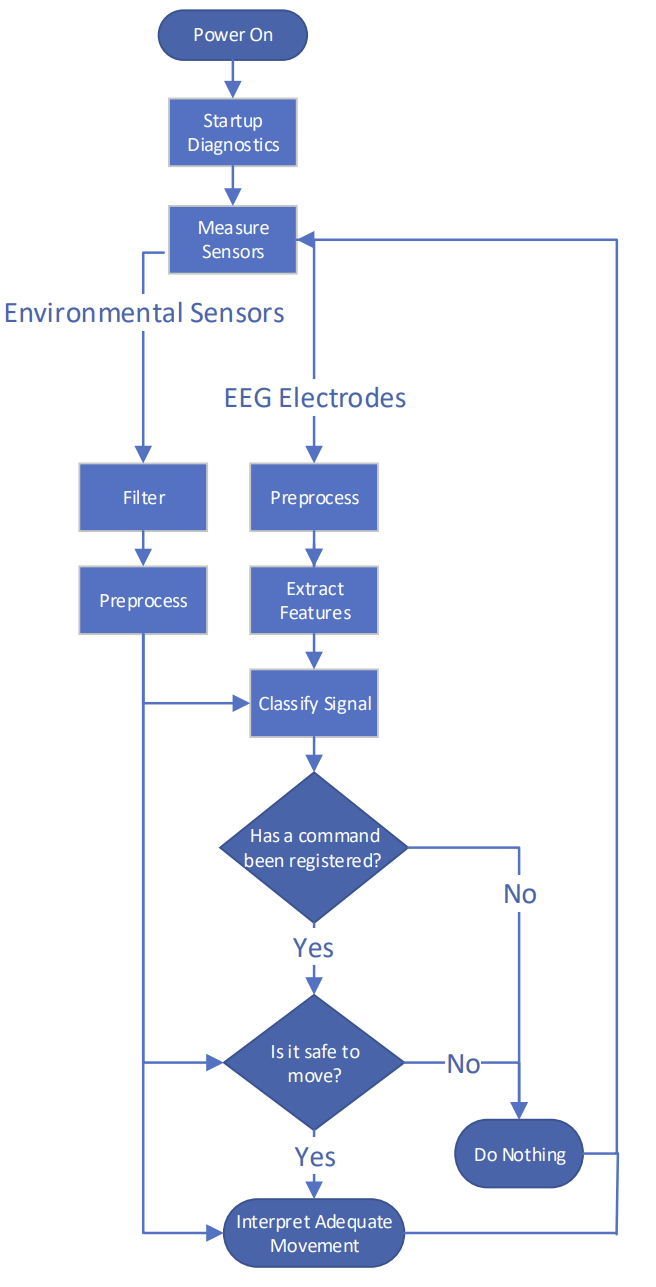
\includegraphics[height=5.1in, keepaspectratio]{figs/D/software-flowchart.png}
            \caption{EEG and Environment Sensor Flowchart}
            \label{fig:eeg_and_sensor}
        \end{figure}
            
        The two data streams follow similar flows and serve as the inputs to the machine learning model. Features such as coherence, power spectral density, and entropy will be calculated from the filtered EEG signal before they are given to the model. The sensor measurements will assist the EEG data in translating the signal into a command. This is a safety measure in the case of a false reading or similar malfunction from the EEG headset. After the model outputs a command, the sensor data will again be used to decide if the chosen direction is one that is safe. If it is determined that the chosen direction and any variation of that direction is not safe for the user, the wheelchair will do nothing. Else, the wheelchair will interpret a precise movement of the wheelchair based on both the output of the model and the surrounding obstacles. 

        \subsubsection{Machine Learning}

        In figure \ref{fig:eeg_and_sensor}, the "Classify Signal" block encapsulates the CNN algorithm used to categorize the signals into one of five commands: forward, backward, left, right, and nothing. The model is shown in Fig. \ref{fig:ml-flow}. It will be structured as a parallel CNN with a concatenation layer. 

         \begin{figure}[htbp]
            \centering
            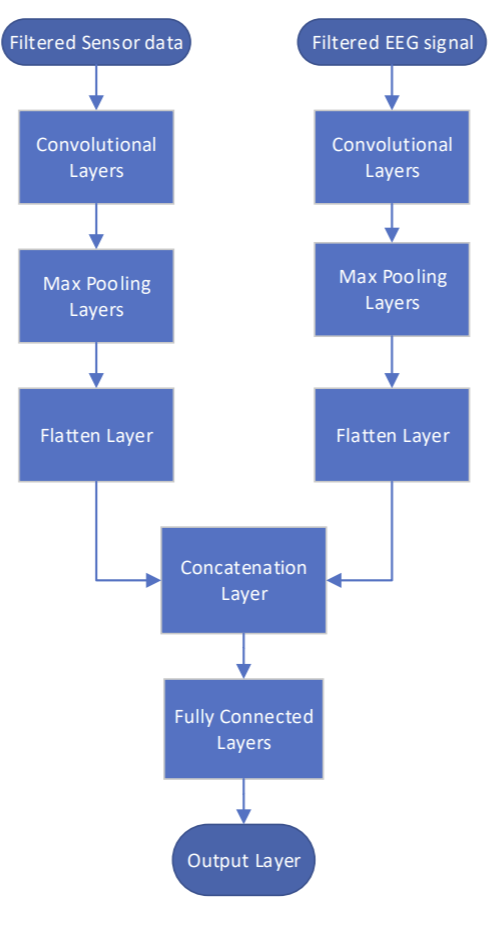
\includegraphics[height=4.7in, keepaspectratio]{figs/ml-flow.png}
            \caption{machine learning Data Flow}
            \label{fig:ml-flow}
        \end{figure}

        After the concatenation layer, the data will be fed into a multi-layered percepetron (MLP) containing an input layer, multiple hidden layers, and an output layer. The resulting output layer will be the weighed outputs for the five commands. 

        \subsubsection{Override and Adjustments}   
        A basic flowchart of the override and adjustment protocol in place is shown in Fig. \ref{fig:override}. This subsection of the system will be instantiated to further ensure reliable wheelchair motion. The flowchart displays the interconnection of the joystick, encoders, and motor drivers. 
         \begin{figure}[htbp]
            \centering
            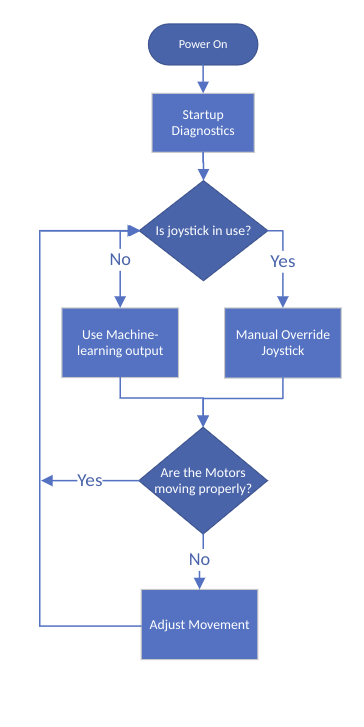
\includegraphics[height=5in, keepaspectratio]{figs/D/override.png}
            \caption{Flowchart of Adjustment and Override Protocol}
            \label{fig:override}
        \end{figure}
        
        The flowchart begins with startup diagnostics. This will detect and attempt to correct joystick drift as well as any malfunctioning of the motors or any other subsystem. Next, joystick use is checked. If no use is detected, machine learning output is used to steer the chair. If use is detected, joystick movement will be mapped to wheelchair movement. The rotary encoders will be used to check proper movement. If the motors are moving as expected, there is nothing to be done and the system loops. If the encoders detect some malfunction, then a signal will be sent to properly adjust the movement of the motors. 

    \subsection{Failure Modes and Effects Analysis}
    Through conducting an FMEA, the team was able to further explore the interconnectivity of the project and any possible associated issues. Potential points of failure that had not been previously discovered were considered, such as the event of a failing stepper motor among others. This analysis is shown in Table \ref{tab:fmea}. In this event, a braking system that can detect fault or failure would be a beneficial safety measure. Additionally, the event of the EEG headset's battery dying is very possible. To counteract this and provide a layer of transparency to the user, the team plans to include a display of the headset's battery percentage on the LCD. This analysis established the importance of having good connections between components, providing the team with valuable insights into potential failure points and how to address them.   

    \onecolumn
    \begin{figure}
        \centering
        \centerline{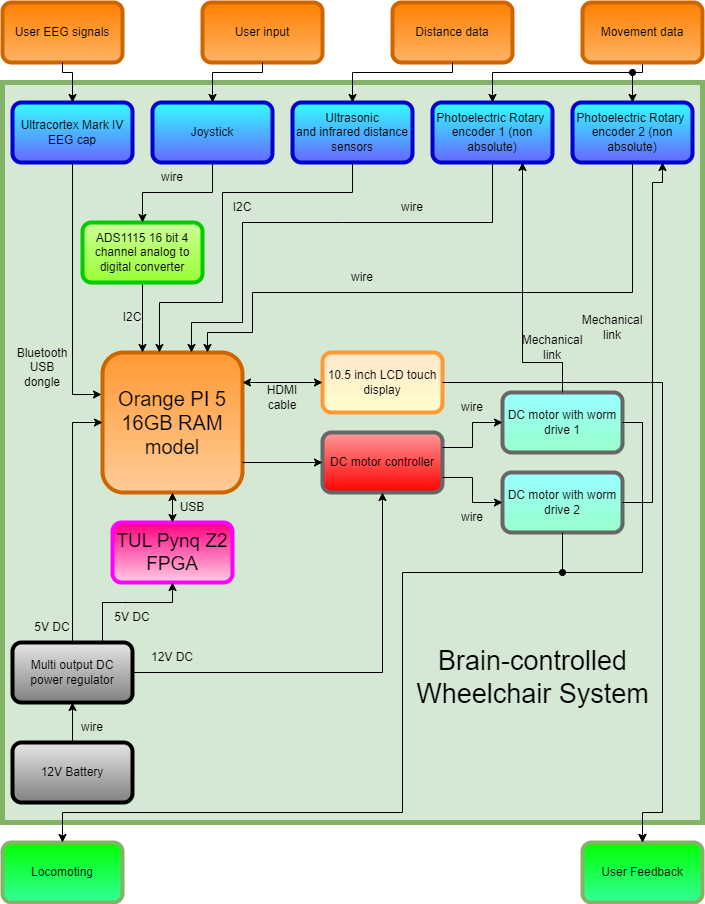
\includegraphics[height=7in, keepaspectratio]{figs/level_2_diagram_1.png}}
        \caption{Level 2 Functional Block Diagram}
        \label{fig:level-2}
    \end{figure}
    
    \begin{table}[htbp]
        \centering
            \begin{tabular}{|>{\columncolor{black!20}}p{0.13\linewidth}|>{\columncolor{black!5}\raggedright\arraybackslash}p{0.10\linewidth}|>{\raggedright\arraybackslash}p{0.12\linewidth}|>{\raggedright\arraybackslash}p{0.15\linewidth}|>{\raggedright\arraybackslash}p{0.15\linewidth}|>{\raggedright\arraybackslash}p{0.05\linewidth} |>{\raggedright\arraybackslash}p{0.14\linewidth}|}
            
            \hline
            \rowcolor{black!20} 
            \textit{\textbf{System}} 
            & \textbf{Components} 
            & \textbf{Failures} 
            & \textbf{Effects} 
            & \textbf{Causes} 
            & \textbf{Severity (0-5)}
            & \textbf{Solutions}\\
            \hline
             & Ultracortex Mark IV 
             & EEG cap loses communication with Orange Pi 5 
             & Wheelchair loses brain-control capability 
             & Dead battery or connection loss 
             & 5 
             & Have a fully charged backup battery on hand and always inspect headset connections before use \\
            \hhline{~------}
            & Joystick 
            & Develops Drift & Wheelchair will move in undesired directions 
            & Wear in the potentiometers 
            & 4 
            & Develop a software protocol to detect and eliminate drift \\
            % \cline{2-7}
            \hhline{~------}
            \multirow{1}{*}{\textit{System Inputs}} 
            & Environmental Sensors 
            & Calculate inaccurate distances 
            & Wheelchair will no longer be able to adjust movement or stop collisions 
            & Becomes dirty, loses connections, environmental changes 
            & 3
            & Always ensure connections are good and make sure sensors are clean \\ 
            % \cline{2-7}
            \hhline{~------}
            & Photoelectric rotary encoders 
            & Do not detect wheel movement 
            & Wheels turn due to external forces. Computer will not be able to detect and stop the wheelchair from moving 
            & Loose connections or dirty photo detector 
            & 3
            & Ensure photo detector is always clean and connections are good \\            
            \hline
            \multirow{4}{*}{\textit{Computing Systems}}
            & Orange Pi 5 
            & Computer malfunctions 
            & Wheelchair will be unresponsive or act uncontrollably 
            & Power loss, loose connections, and/or software error 
            & 4
            & Ensure power systems and all other connections are firmly connected and make sure software is up to date and working correctly \\
            % \cline{2-7}
            \hhline{~------}
            & TUL Pynq Z2 
            & Computer malfunctions 
            & EEG signals may not be interpreted correctly and stop or product undesired movement 
            & Power loss, loose or bad USB cable 
            & 4
            & Ensure software is robust, ensure physical connections are attached properly \\
            \hline 
            & Motor drivers 
            & Loss of function 
            & Wheelchair will no longer have controlled movement 
            & Power loss, power overdraw from strain, or misuse 
            & 5
            & Make sure all connections are good and power delivery system is in working order \\
            % \cline{2-7}
            \hhline{~------}
            \multirow{2}{*}{\textit{System Outputs}} 
            & DC Motors with Worm Drive 
            & Loss of function 
            & Wheelchair will not move under command and have no means of braking 
            & Power loss, power overdraw, or loose connections 
            & 5
            & Ensure motor specs, ensure secure connections \\
            % \cline{2-7}
            \hhline{~------}
            & LCD 
            & Display goes black 
            & User will not have visual indication if the chair is working and moving correctly 
            & Loose connection or misuse 
            & 3
            & Make sure the cable is connected securely and the display is secure to the chair\\
            \hline
        \end{tabular}           
        \caption{Failure Modes and Effects Analysis}
        \label{tab:fmea}
    \end{table}
    \twocolumn


%%%%%%%%%%%%%%%%%%%%%%%%%%%%%%%%%%%%%%%%%%%%%%%%%%%%%%%%%%%%
\clearpage
\onecolumn
\begin{center}
    \addcontentsline{toc}{section}{Appendix E}
    \vspace*{5cm}
     {\Huge\bfseries Appendix E \par}
     \vspace{1cm}
    \textit{Final Design} \\
\end{center}
\clearpage
\twocolumn

\setcounter{section}{5}
\renewcommand{\thesubsection}{E.\Alph{subsection}}
\section*{\textbf{Appendix E}}
        \setcounter{figure}{0}
        \renewcommand{\thefigure}{E.\arabic{figure}}
        \setcounter{table}{0}
        \renewcommand{\thetable}{E.\arabic{table}}
        \setcounter{subsection}{0}
        
    \subsection{Bill of Materials}
    The current bill of materials is displayed in Table \ref{tab:final_design_bom}, showing components that will be used to construct and implement the final design. It is worth noting that while this list covers the important parts, some additional components may be needed during the testing and building process. The wheelchair is not included in the table as the team has not yet devised an adequate plan of action to implement the design. As mentioned earlier in the report, there are some upgrades to be considered with the design involving the minicomputer. The current minicomputer, the Orange Pi 5, does not have WiFi or Bluetooth build into the motherboard, relying on external connections to achieve the functionality. The upgrade to this minicomputer, the Orange Pi 5B, has these features included on the motherboard. This will be beneficial for the implementation of the system for communication of the machine learning inputs and outputs to the remote server via WiFi and for Bluetooth communication with the Ultracortex EEG cap. 


    \begin{table}[htbp]
        \centering
        
        \begin{tabular}{|>{\raggedright\arraybackslash}p{0.30\linewidth}|>{\raggedright\arraybackslash}p{0.15\linewidth}|>{\raggedright\arraybackslash}p{0.12\linewidth}|>{\raggedright\arraybackslash}p{0.18\linewidth}|}
            
            \hline
            \rowcolor{black!20} 
            {\textbf{Part Name}} 
            & \textbf{Price} 
            & \textbf{Quantity} 
            & \textbf{Total Cost} 
            \\
            \hline

            \rowcolor{black!10}
            OpenBCI Ultracortex Mark IV & \$ 3449.99 & 1 & \$ 3449.99 \\

            \rowcolor{black!5}
            Orange Pi 5 16GB & \$ 130.99 & 1 & \$ 130.99 \\

            % \rowcolor{black!10}
            %  Standard Wheelchair & \$ 145.79 & 1 & \$ 145.79 \\


            \rowcolor{black!10}
              Roboclaw 2x7A Motor Controller & \$ 79.95 & 1 & \$ 79.95 \\

            \rowcolor{black!5}
             Ultrasonic Sensor 5 Pack & \$ 11.39 & 1 & \$ 11.39 \\

            \rowcolor{black!10}
             Infrared Sensor 6 Pack & \$ 6.99 & 1 & \$ 6.99 \\

            \rowcolor{black!5}
             Wishiot IMU-60-50 & \$ 13.99 & 1 & \$ 13.99 \\

            \rowcolor{black!10}
             Joystick & \$ 6.29 & 1 & \$ 6.29 \\

            \rowcolor{black!5}
             ADS1115 16-bit 4-channel ADC & \$ 7.99 & 1 & \$ 7.99 \\

            \rowcolor{black!10}
             Photoelectric non absolute rotary encoder 5 pack & \$ 7.29 & 1 & \$ 7.29 \\

            \rowcolor{black!5}
             12V to 5V 50W buck converter & \$ 15.99 & 1 & \$ 15.99 \\

             \rowcolor{black!10}
             12V power supply & \$ 249.98 & 1 & \$ 249.98 \\

            \rowcolor{black!5}
             Arduino RC Car Kit Base & \$ 18.99 & 1 & \$ 18.99 \\

             \rowcolor{black!10}
              RF24L01 & \$ 8.49 & 1 & \$ 8.49 \\

              \rowcolor{black!5}
              DC motor with worm drive & \$ 29.99 & 2 & \$ 59.98 \\

              \rowcolor{black!10}
              TUL Pynq Z2 FPGA & \$ 123.00 & 1 & \$ 123.00 \\

            \rowcolor{black!5}
              Orange Pi LCD Display & \$ 81.99 & 1 & \$ 81.99 \\

     
            \hline
            \rowcolor{black!20} 
            {\textbf{Within initial budget of \$7,550.00? }} 
            & \textbf{Yes} 
            & \textbf{Total} 
            & \textbf{\$ 4419.08} 
            \\
            \hline
        \end{tabular}

        \caption{Bill of Materials}
        \label{tab:final_design_bom}
    \end{table}    
    
    \subsection{Schematics}
    A schematic of the system is shown in Fig. \ref{fig:schematic}. This schematic includes all of the components mentioned in the bill of materials and displays where and how they are connected. The components include two computing modules: the Orange Pi 5 and the TUL Pynq Z2. The Orange Pi 5 acts as the conductor of the system, offloading repetitive machine learning calculations to the TUL Pynq Z2 and controlling wheelchair movement by taking in sensor and user input and outputting to the motor drivers. Both devices receive 5V power from a 12V to 5V DC buck converter.

    The remainder of the system is divided into four subsystems: environmental, locomotion, power, and user input. The environmental subsystem includes four infrared sensors, four ultrasonic sensors, and an IMU. Ultrasonic and infrared sensors communicate with the Orange Pi 5 via GPIO ports, while the IMU communicates via I2C. These sensors assist the wheelchair in making decisions about movement at two stages. The sensors serve as inputs to the machine learning model as shown in \ref{fig:eegnet} and are monitored before final output is sent to the motor drivers as shown in \ref{fig:eeg_and_sensor}. 

    The locomotion subsystem includes DC motor controllers, DC motors with worm drives, and photoelectric rotary encoders. The Orange Pi 5 communicates the desired movement to the DC motor controller via GPIO pins, which controls the speed of the motors. The motor controller uses a closed-loop system with photoelectric encoders to adjust the motor speed. The motor controller is connected to the 12V battery terminals on the motor connection side and a 5V supply on the input side. The photoelectric encoders connect to the EN1 and EN2 ports of the controller. Prior to connecting to the Orange Pi 5, the motor controller can be calibrated using the software available on the Roboclaw \cite{roboclaw} website.

    The power subsystem includes a 12V battery, 12V to 5V DC buck converter, and various cabling and adapters. The Orange Pi 5, LCD display, and TUL Pynq Z2 connect to the 5V supply of the buck converter via USB Type-C adapters. Devices that require 5V supply receive it through the V5 GPIO pins of the Orange Pi 5. Only the 12V power side of the motor controller is wired directly to the battery.

    The user input subsystem includes the OpenBCI Ultracortex Mark IV EEG cap and manual override joystick. The Ultracortex Mark IV EEG cap has its battery power supply and communicates with the Orange Pi 5 via a USB Bluetooth dongle. The manual override joystick connects to the 5V and GND GPIO pins of the Orange Pi 5. Analog signals from the joystick go into the A0 and A1 ports of an analog-to-digital ADS1115 converter that transmits joystick readings to the Orange Pi 5 via I2C. 
    
    \subsection{Software Design}
    This section will build off of what was already mentioned by earlier sections of the report, but will hone in on specific design choices where earlier sections have not gone into detail. The two sections of focus will be the specific machine learning model and the process of the startup diagnostics. 
    
    \subsubsection{Machine Learning}
    Table \ref{tab:ml-tbl} mentions the various machine learning models considered by the team after reviewing related work from \cite{a_comprehensive_review, dmtl_bci, eegnet, eegnet_processor_design, lstm_eeg, robotic_architecture, toward_brain_computer, deep_learning_eeg} and speaking with experts in both machine learning and EEG signal analysis. The team has decided to use EEGNet \cite{eegnet}, as it has been documented to perform well in applications of recognizing motor imagery commands from EEG signals, is lightweight and portable, and has been successfully implemented directly in hardware \cite{deep_learning_eeg, eegnet_processor_design}. The code for this model has also been published by the authors and is free to access on GitHub. A visualization of the network can be found in \ref{fig:eegnet}. Being a derivative of the CNN, EEGNet is comprised of convolutional layers which flatten the incoming signals that are then fed as inputs into an MLP. The model will be akin to that of what is detailed in \cite{eegnet}, however will contain the additional inputs of the environmental sensor data from the infrared sensors, ultrasonic sensors, and IMU. The network starts by deconstructing the signals into their respective frequency bands, then performs depth-wise convolution to learn frequency-specific spatial filters. This is followed by both signals undergoing separable convolution which learns a temporal summary for each feature map individually. Before being fed into the MLP, the signals are pointwise convoluted, which is a process that learns how to optimally mix the feature maps together. 
    
    \subsubsection{Startup Diagnostics}
    A finite state machine (FSM) of the startup diagnostics is shown in Fig. \ref{fig:initial_diag}. The FSM represents the software that will run upon the system being powered on and will ensure that the user input and environmental subsystems are properly functional and do not hinder wheelchair operation. Some noteworthy checks that the FSM considers are functionality of EEG electrodes, proper connection of EEG electrodes to the user's scalp, functionality of environmental sensors, and accuracy of the environmental sensors. If any of these subsystem experiences unknown behavior, then the error will be reported to the user through display on the LCD. The user will either be prompted to quickly fix the problem or if the error is severe and will not allow the wheelchair to operate safely, the system will exit. 

    \subsection{Assembly}
    The following instructions pertain to the schematic of the system and do not include details to the RC car test rig or wheelchair implementation. Refer to the schematic in Fig. \ref{fig:schematic} for more detail. 

    \begin{enumerate}
        \item Power
        \begin{itemize}
            \item Beginning with the battery, connect two wires to the positive and negative terminals each. The wires of connected to the positive terminal should be red and likewise the wires connected to the negative terminal should be black.
            \item Connect once set of red and black wires to the red and black wires of the DC buck converter and the other set of red and black wires to the battery input of the DC motor controller.
            \item From the DC buck converter attach yellow and black wires to the yellow and black wire output of the DC buck converter. This cable will have three USB type C adapters.
            \item Plug each of the USB C adapters into the USC C power port on the Orange Pi 5 and do likewise for the TUL Pynq Z2, and LCD display.
        \end{itemize}
        \item Computing
        \begin{itemize}
            \item Connect the USB cable between the Orange Pi 5 and TUL Pynq Z2
            \item Plug in the USB dongle for the Ultracortex Mark IV EEG cap.
        \end{itemize}
        \item Environmental Sensors
        \begin{itemize}
            \item Wire all the trigger wires of the four ultrasonic sensors together and connect them the proper GPIO port of the Orange Pi 5 using the schematic in Fig. \ref{fig:schematic}.
            \item Wire all the echo pins to the correct GPIO pins using the schematic as before.
            \item Connect the VCC and GND pins of each ultrasonic sensor to the 5V and GND pins of the Orange Pi 5 GPIO headers. Refer to schematic for help.
            \item For the infrared sensors, connect all the VCC and GND pins to the same 5V and GND pins of the Orange Pi 5 as you did in the previous instruction.
            \item Wire the out pin from each infrared sensor to the correct GPIO pin of the Orange Pi 5 using the schematic.
            \item Connect the VCC and GND pins of the IMU to the same as the previous set.
            \item Referring to the schematic, connect the SCL and SDA wires of the IMU to the correct GPIO pins of the Orange Pi 5.
        \end{itemize}
        \item Locomotion
        \begin{itemize}
            \item Connect the VCC and GND pins of the DC motor controller to the Correct GPIO pins of the Orange Pi 5 using the schematic.
            \item Connect the VCC and GND pins of each photoelectric encoder to the same 5V and GND connectors from the Orange Pi 5. 
            \item Connect the EN 1 and EN2 pins to the out pins of the photoelectric encoders.
            \item Connect the red wires from each motor to separate +12V screw terminals of the DC motor controller.
            \item Connect the black wires of each motor to the GND screw terminals of the DC motor controller.
        \end{itemize}
        \item User Interface
        \begin{itemize}
            \item Connect the joystick VCC and GND pins to the corresponding 5V and GND GPIO pins of the Orange Pi 5.
            \item Connect the VRX pin of the joy stick to the A0 pin and the VRY pin to A1 of the ADS1115. 
            \item Connect the VCC and GND pins to the 5V and GND GPIO pins of the Orange Pi 5.
            \item Connect the SCL and ADS pins to the same corresponding GPIO pins of the Orange Pi 5 as the IMU.
            \item Next connect the LCD display to the Orange Pi 5 using an HDMI cable.
            \item Finally, power on and put on the Ultracortex Mark IV EEG cap.
        \end{itemize}
    \end{enumerate}
    
    \subsection{Operational Gantt Chart}

    An updated Gantt chart is shown in Fig \ref{fig:updated_gantt}. The chart assigns tasks to team members and specifies the duration of their work on each task. By using this chart, the team aims to keep the remaining aspects of the project organized to maintain a consistent and productive workflow. It is the team's belief that by following this approach, the project will be completed successfully in a timely manner. 

    The team is committed to following the Operational Gantt Chart strictly in order to complete the project and allow sufficient time for testing and construction of the mock wheelchair. The team's goal is to go beyond the proof-of-concept brain-controlled RC car and to build a fully functioning wheelchair controlled by the user's thoughts. Durring the summer months, work will focus on software development and construction of the RC car testing rig. Once the rig is built, the team will continuously improve the functionality and performance of the system. When the system reaches a sufficient state, the design and construction of the wheelchair will commence. 

    \onecolumn
    \begin{figure}
        \centering
        \centerline{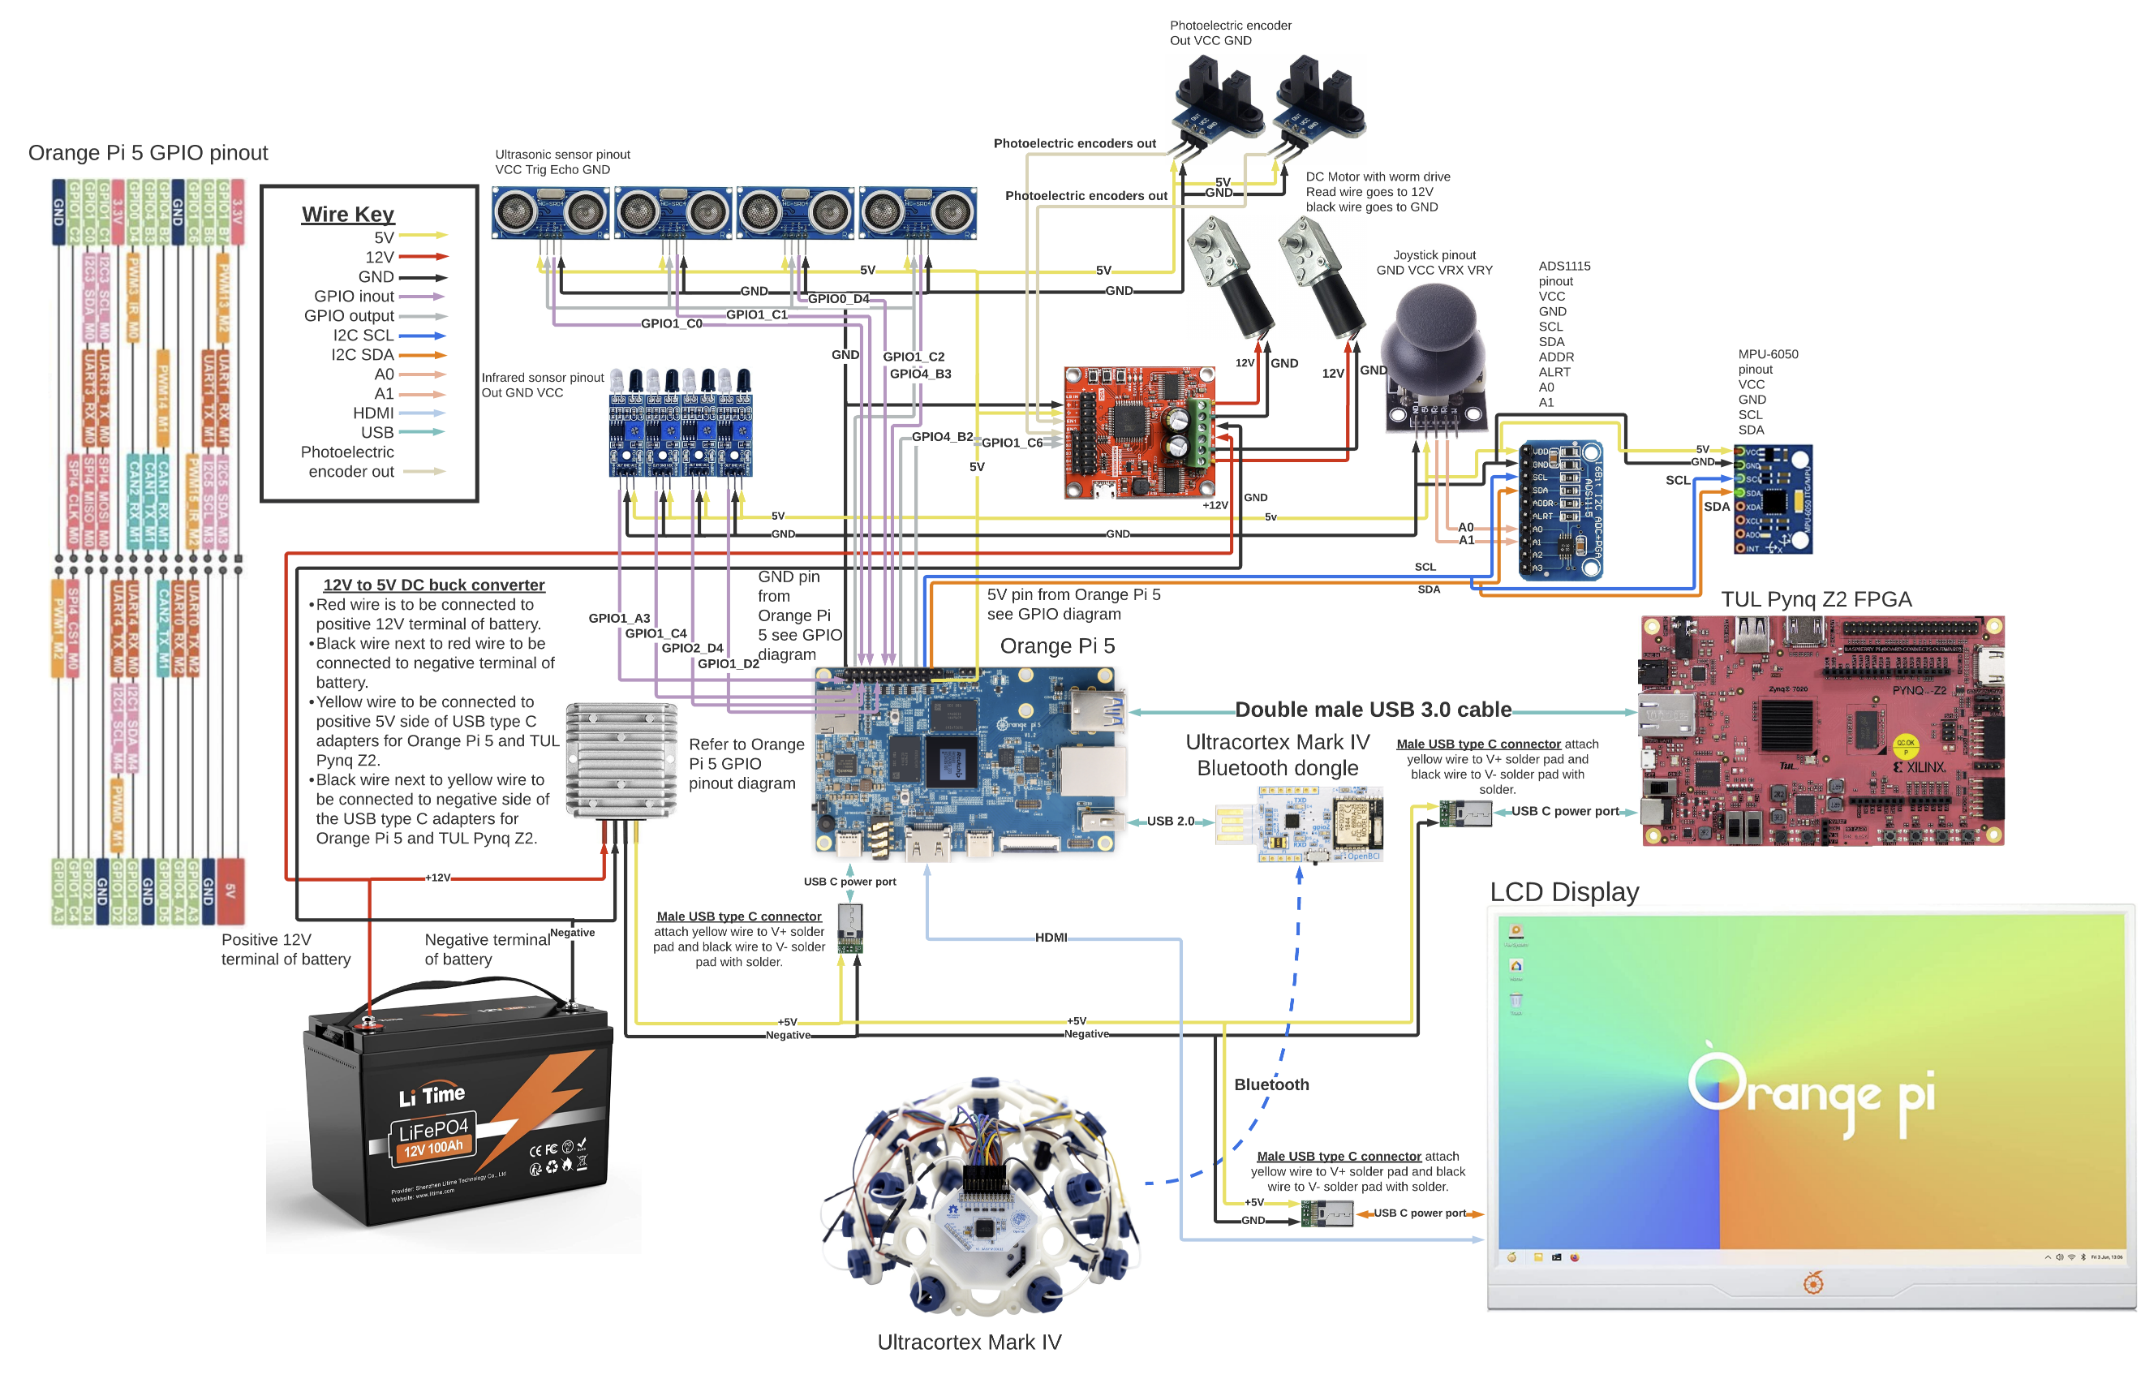
\includegraphics[angle=90,height=9in, keepaspectratio]{figs/E/schematic.png}}
        \caption{Schematic of Brain-Controlled Wheelchair}
        \label{fig:schematic}
    \end{figure}
    \twocolumn

    \onecolumn
    \begin{figure}
        \centering
        \centerline{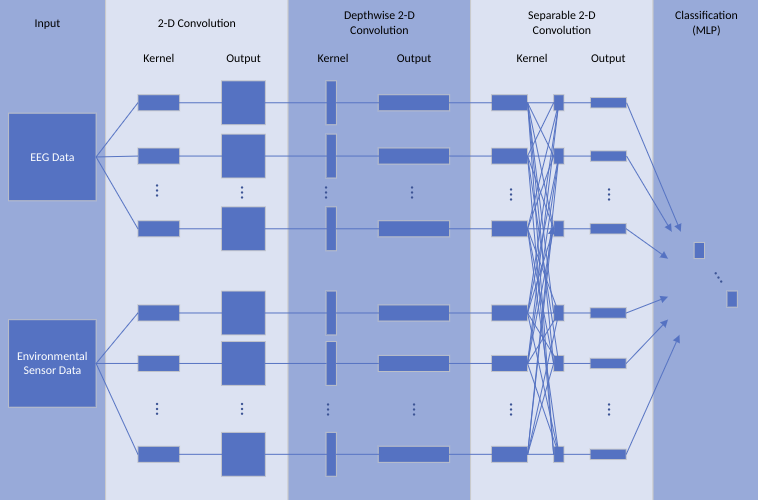
\includegraphics[height=4in, keepaspectratio]{figs/E/eegnet.png}}
        \caption{Visualization of EEGNet}
        \label{fig:eegnet}
    \end{figure}
    \begin{figure}
        \centering
        \centerline{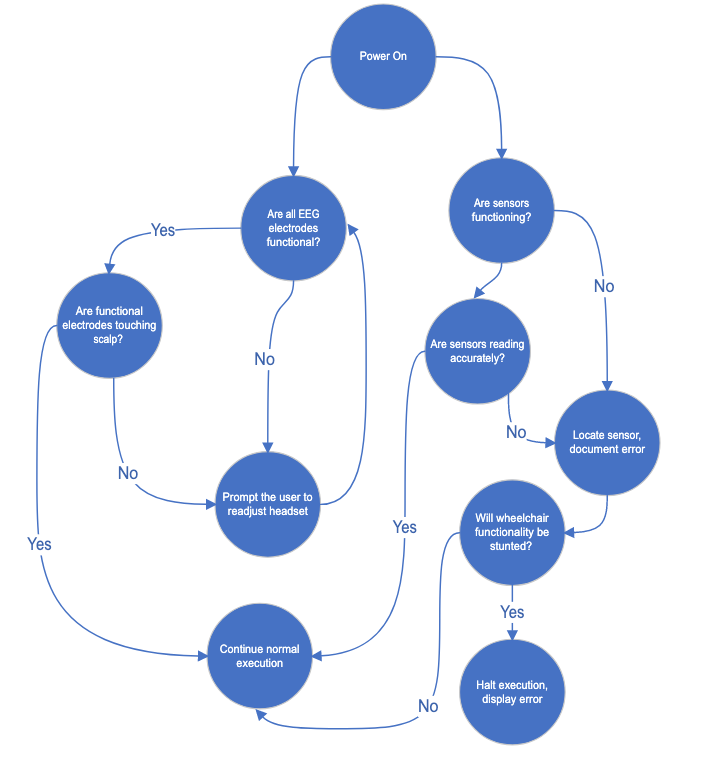
\includegraphics[height=4in, keepaspectratio]{figs/E/initial_diag_fsm.png}}
        \caption{Startup Diagnostics Finite State Machine}
        \label{fig:initial_diag}
    \end{figure}
    \twocolumn
    
    \onecolumn
    \begin{figure}
        \centering
        \centerline{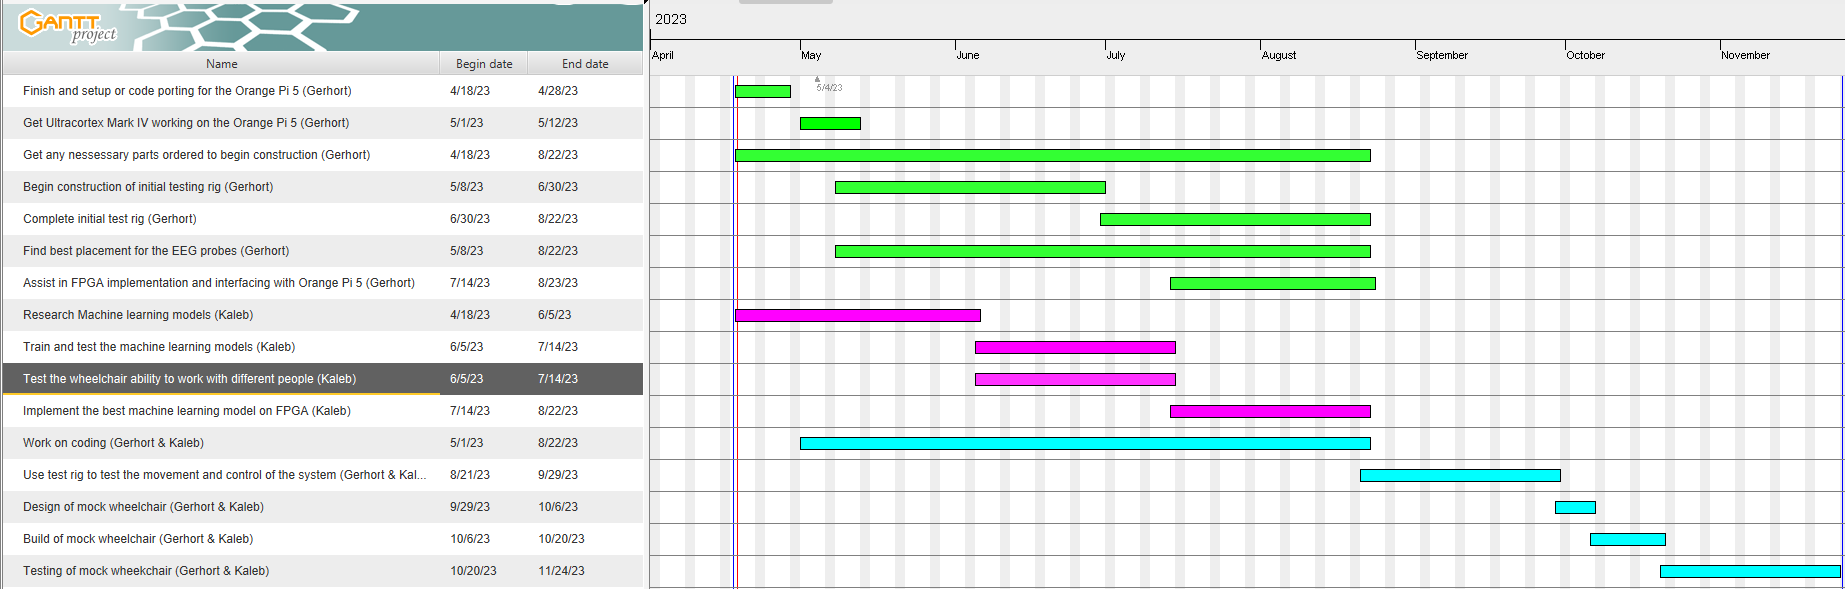
\includegraphics[angle=90,height=8.5in, keepaspectratio]{figs/E/updated_gantt.png}}
        \caption{Updated Gantt Chart}
        \label{fig:updated_gantt}
    \end{figure}
    \twocolumn





    
\end{document}
